\documentclass{article}   
\usepackage[left=1.5cm,right=1.5cm,top=2.3cm,bottom=2.3cm]{geometry}		
\usepackage[utf8]{inputenc} 										
%\usepackage[french]{babel}
\usepackage{fancyhdr}								
\usepackage{hyperref}
\hypersetup{
    colorlinks=true,        % false: boxed links; true: colored links
    linkcolor=black,         % color of internal links (e.g., sections)
    citecolor=black,         % color of citation links
    filecolor=black,         % color of file links
    urlcolor=black           % color of external links
}								
\usepackage{booktabs,multirow,hhline}		
\usepackage{graphicx}				
\usepackage{bibentry}
%\usepackage{wrapfig,caption}
\usepackage{subcaption}
\usepackage[compact]{titlesec}
\titlespacing{\section}{0pt}{2ex}{1ex}
\titlespacing{\subsection}{0pt}{1ex}{0ex}
\titlespacing{\subsubsection}{0pt}{0.5ex}{0ex}
\usepackage{color}												
\usepackage[dvipsnames]{xcolor}								
\usepackage{amsmath,amssymb,amsthm,nicefrac}
\usepackage{mathrsfs}										
\usepackage{wasysym,marvosym}
\usepackage{mathtools}
\usepackage{verbatim}										
\usepackage{minted}										
\usepackage{lipsum}
\usepackage{tikz}
\usetikzlibrary{calc,patterns,angles,quotes}
\usepackage[american]{circuitikz}
\usepackage{siunitx}
\usepackage{physics}
\usepackage{float}
\usepackage{movie15}
\usepackage{multicol}
\usepackage{lineno}

\captionsetup[figure]{font=footnotesize, labelfont=bf}
\captionsetup[table]{font=footnotesize, labelfont=bf}

%\usepackage[backend=biber, style=numeric]{biblatex}
%\addbibresource{references.bib} %Imports bibliography file
\usepackage[super,sort]{natbib}

\renewcommand{\textfraction}{0.001} % Allows minimal text on a page
\renewcommand{\floatpagefraction}{0.999} % Requires float pages to be nearly full
\renewcommand{\topfraction}{0.999} % Allows the top of the page to be nearly all float
\renewcommand{\bottomfraction}{0.999} % Allows the bottom of the page to be nearly all float
\setcounter{totalnumber}{5}  % Maximum number of floats on a text page
\setcounter{topnumber}{3}    % Maximum number of floats at the top
\setcounter{bottomnumber}{2} % Maximum number of floats at the bottom

\parindent=0pt									
\parskip=6pt

\fancyheadoffset{0 cm}	

\linenumbers

%-------------------------------------------------------------------------------------------

\begin{document}

\begin{center}

    {\Large \textbf{Emergence of geometric functional connectivity gradients in spatially embedded neuronal networks}}\\
    
    \vspace{10 pt}
    \textbf{Antoine Légaré},$^{1,2}$ \textbf{Olivier Ribordy},$^{3,4}$, \textbf{Paul De Koninck}$^{1,2}$, \textbf{Antoine Allard},$^{3,4,*}$ \textbf{Patrick Desrosiers},$^{1,3,4,*}$ \\
    \vspace{5 pt}
    
    $^1$\textit{Centre de recherche CERVO, Québec (Qc), Canada.}\\
    $^2$\textit{Département de biochimie, de microbiologie et de bio-informatique, Université Laval, Québec (Qc), Canada}\\
    $^3$\textit{D\'epartement de physique, de g\'enie physique et d'optique, Universit\'e Laval, Qu\'ebec (Qc), Canada}\\% G1V 0A6}
    $^4$\textit{Centre interdisciplinaire en mod\'elisation math\'ematique de l'Universit\'e Laval, Qu\'ebec (Qc), Canada}\\
     $^*$\textit{Co-corresponding authors:} \href{mailto:patrick.desrosiers@phy.ulaval.ca}{patrick.desrosiers@phy.ulaval.ca}; \href{mailto:antoine.allard@nphy.ulaval.ca}{antoine.allard@phy.ulaval.ca}

\end{center}

\vspace{4 pt}

\hrulefill

\textbf{Abstract} - The geometry of the brain imposes fundamental constraints on its activity and function. However, the mechanisms linking brain shape to neuronal dynamics remain elusive. Here, we investigate how geometric eigenmodes relate to functional gradients of neuronal activity within three-dimensional structures using numerical simulations and calcium imaging experiments in larval zebrafish. We show that functional gradients arising from network activity closely match the geometric eigenmodes of the network’s spatial embedding when neurons are locally connected. By systematically varying network parameters such as the connectivity radius and the prevalence of long-range connections introduced via edge swaps, we reveal a robust geometry-function correspondence that progressively deteriorates as local connectivity is disrupted. Additionally, we demonstrate that spatial filtering can artificially impose geometric structure on functional gradients, even at modest levels. To support our computational results, we conduct volumetric calcium imaging experiments at cellular resolution in the optic tectum of zebrafish larvae. We uncover cellular functional gradients that closely align with geometric eigenmodes up to a certain mode wavelength that reflects the spatial extent of neuronal arborizations measured in single-neuron reconstructions, as predicted by our simulations. Our findings highlight the importance of short-range anatomical connectivity in shaping the spatial structure of brain activity.

\hrulefill
\vspace{10 pt}

%\begin{multicols}{2}

\section*{Introduction}

Brain activity during wakefulness is continuous and exhibits complex spatiotemporal patterns. Understanding what shapes the flow of brain-wide activity remains a central challenge in systems neuroscience. At any given moment, several factors influence brain activity, including external sensory inputs or ongoing internal demands\cite{flavell2022emergence}. However, the brain’s structural connectivity imposes perhaps the most fundamental constraint on its dynamics\cite{suarez2020linking}. As in many natural systems, structure and function in the brain are deeply intertwined. Synaptic wiring diagrams can predict patterns of coordinated activity across neurons\cite{uzel2022set, randi2023neural, lappalainen2024connectome} and brain regions\cite{legare2024structural}, while the spatial organization of neural populations across gyri, sulci, and subcortical nuclei reflects their functional specialization. A comprehensive understanding of how activity flows through the brain must therefore integrate both its network architecture and its spatial embedding—--its geometry.

In human neuroimaging, network science is widely employed to model both anatomical connectivity and brain dynamics\cite{bassett2017network}. The most common network-based description of brain activity is functional connectivity (FC), typically defined as the correlation between activity time series from distinct brain regions. Although FC provides a compact summary of interactions between neuronal populations over extended periods, it fails to describe the brain’s rapid, moment-to-moment fluctuations\cite{zamani2020high}. Nonetheless, FC has proven useful: it reflects effective connectivity and is correlated with structural connectivity (SC), a relationship referred to as the structure-function coupling of brain networks\cite{fotiadis2024structure}. A recent and influential extension of FC analysis is the use of functional connectivity gradients---spatially continuous eigenvectors that capture the dominant axes of variation in connectivity profiles\cite{margulies2016situating, huntenburg2018large, bernhardt2022gradients}. These gradients have become powerful tools to examine the spatial organization of brain functions, not only in humans but also in animal models such as mice and zebrafish\cite{coletta2020network, legare2024structural}. While gradient analysis inherits the static nature of the FC matrix, the resulting spatial configurations offer insights into underlying dynamical processes. In particular, recent work has shown that a large portion of FC variance is driven by propagating waves of hemodynamic activity, which diffuse along canonical resting-state networks (RSNs) organized along the functional gradients\cite{yousefi2021propagating, raut2021global}. Thus, FC and its gradients appear to reflect the influence and directionality of spatially propagating activity, yet the mechanisms shaping these patterns remain incompletely understood.

Across a wide range of recording modalities and animal models, waves of neuronal activity have been consistently observed in both cortical and subcortical structures\cite{raut2021global, ye2023brain, matsui2016transient, xu2023interacting}. While their precise origins and computational roles remain debated, these waves likely emerge from fundamental architectural features such as conduction delays and the prevalence of short-range connectivity\cite{muller2018cortical}. A hallmark of brain networks is wiring length minimization, which favors local connections between neurons or brain regions\cite{bullmore2012economy}. Although long-range projections are essential to coordinate global dynamics\cite{o2013causal, betzel2018specificity, vohryzek2025human}, their relative sparsity suggests that much of brain activity arises from local interactions. Neural Field Theory (NFT) formalizes this idea by modeling brain activity as the propagation of electrical waves across a continuous neural sheet\cite{robinson1997propagation, robinson2016eigenmodes, gabay2018dynamics}, typically governed by an exponential decay rule (EDR) of connectivity\cite{ercsey2013predictive}. A recent study by Pang and colleagues\cite{pang2023geometric} used noninvasive MRI to test a key prediction of NFT: that cortical geometry itself imposes constraints on activity propagation beyond those imposed by white matter connectivity. Supporting this hypothesis, they showed that geometric eigenmodes of the cortical surface offer a parsimonious basis to reconstruct brain activation patterns\cite{pang2023geometric}. Remarkably, a one-to-one correspondence was observed between geometric eigenmodes and FC gradients in subcortical structures, where shape alone predicted the dominant axes of functional organization\cite{pang2023geometric}. These findings underline the strong influence of geometry on brain function, yet the generative mechanisms linking geometry, connectivity, and activity remain elusive. Moreover, the limited spatial resolution of fMRI, together with common preprocessing steps such as spatial filtering, can introduce biases in gradient analyses\cite{watson2023connectopic}, underscoring the need for validation in alternative animal models where such confounds are absent.

In this study, we combine numerical simulations and optical imaging in the larval zebrafish at cellular resolution to investigate the link between functional gradients and geometric eigenmodes in brain networks. Using simulations of neuronal networks embedded in various 3D shapes, we show that the correspondence between gradients and eigenmodes emerges naturally from short-range connectivity and local correlations, independent of specific spatiotemporal dynamics. We further demonstrate that this mapping deteriorates as local connectivity is disrupted, revealing a wavelength-dependent decay of the eigenmode-gradient correspondence that serves as a sensitive readout of the spatial extent of underlying anatomical connections. To validate our numerical findings and extend previous neuroimaging results\cite{pang2023geometric}, we perform two-photon calcium imaging in the larval zebrafish optic tectum, where we observe functional gradients that coincide with the structure’s geometry. Consistent with our simulations, the cutoff point of this geometric mapping predicts the median arbor size of reconstructed tectal neurons with micron-level precision\cite{kunst2019cellular}. Collectively, our results uncover a simple generative mechanism for the emergence of geometric connectivity gradients in the brain and underscore the prevailing influence of geometry on both anatomical wiring and functional organization.

\section*{Results}

Throughout this study, we compare geometric eigenmodes and FC gradients (hereafter referred to as eigenmodes and gradients, respectively) in neuronal populations embedded within various three-dimensional shapes. Geometric eigenmodes are the eigenvectors of the Laplace–Beltrami operator (LBO, see Methods), and capture spatial patterns---analogous to vibrational modes---that arise from the shape of the embedding. FC gradients are computed from pairwise activity correlations using diffusion maps\cite{Coifman2006}, and represent principal axes of connectivity variation in the network (see Methods). When applied to brain connectivity data, functional gradients spatially map onto different brain functions, providing a data-driven measure of functional organization\cite{margulies2016situating}.

\subsection*{Functional gradients and geometric eigenmodes in locally connected networks}

\begin{figure*}[t]
    \centering
    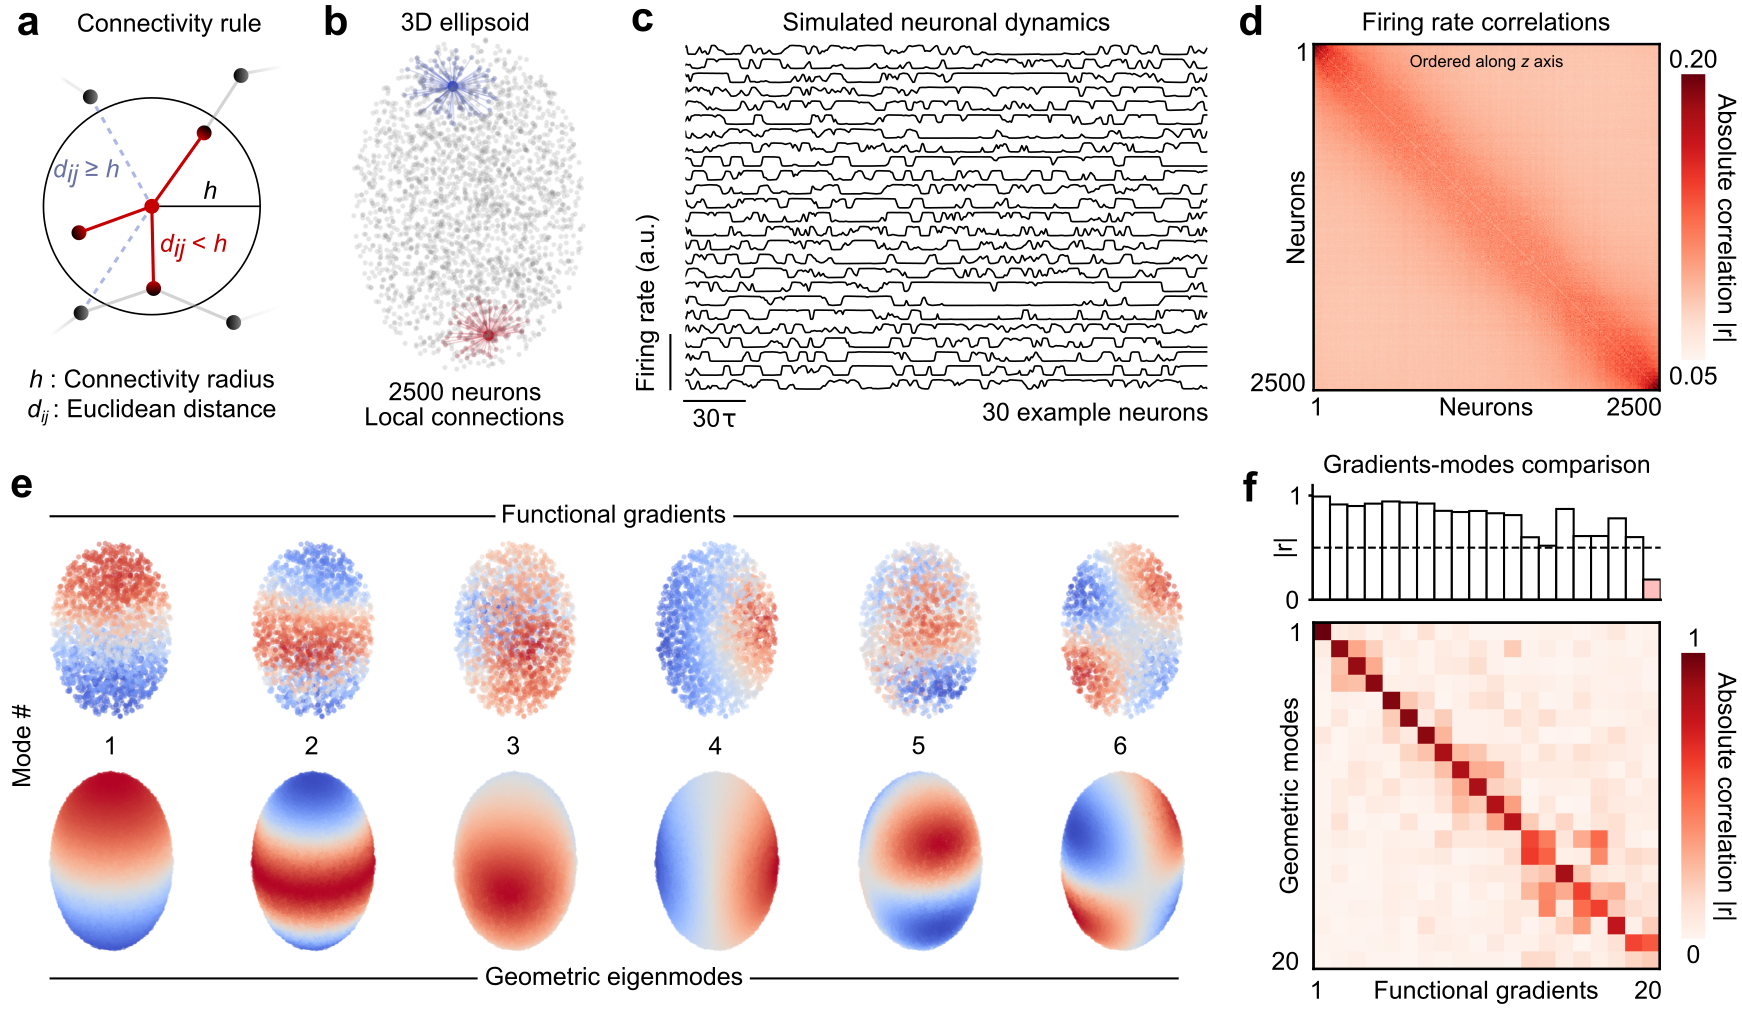
\includegraphics[width=1.0\linewidth]{figures/figure1.png}
    \caption{Geometric gradients emerge in firing rate networks with local connectivity. (\textbf{a}) Visualization of the connectivity rule, wherein two nodes are connected if and only if separated by Euclidean distance less than $h$. (\textbf{b}) Centroids of 2500 neurons in a 3D ellipsoid; example local connectivity profiles with $h=0.1$ are highlighted in red and blue. (\textbf{c}) Example firing rate dynamics from 50 neurons in one simulation. (\textbf{d}) Average correlation matrix from 250 simulations; neurons are ordered along the $z$ major axis of the ellipsoid. (\textbf{e}) Top row, six functional gradients obtained using diffusion eigenmap, ordered based on their similarity with geometric modes; bottom row, first six geometric eigenmodes of the ellipsoid, with the first constant mode excluded. (\textbf{f}) Bottom, absolute correlation matrix of the first 20 gradient-mode pairs, after functional gradients have been optimally mapped to geometric modes; top, absolute correlations of the optimally mapped modes (diagonal of the matrix below); a dashed line indicates an intermediate $|r|=0.5$ correspondence.}
    \label{fig1}
    \hrulefill
\end{figure*}

To understand the relationship between gradients and eigenmodes, we first simulated neuronal population dynamics in various three-dimensional geometries. Neurons were assigned random coordinates within a volume, then connected if separated by a distance $d_{ij}<h$, where $h$ is a threshold we refer to as the network's connectivity radius (Fig. \ref{fig1}\textbf{a}). As a first case, we generated a simple 3D ellipsoid with $N=2500$ locally connected neurons within a radius $h=0.1$, corresponding to 10\% of the system’s characteristic length (Fig. \ref{fig1}\textbf{b}). We simulated simple chaotic firing rate dynamics resulting from nonlinear excitatory and inhibitory interactions between connected neurons (Fig. \ref{fig1}\textbf{c}, Methods). We then computed an average absolute correlation matrix $C$ from the firing rates of neurons by averaging the correlations from 100 simulations, throughout which node coordinates and connections were preserved, but connections weights and initial conditions were drawn randomly each time. Correlations were generally higher between neurons situated at roughly the same position along the vertical axis of the ellipse (Fig. \ref{fig1}\textbf{d}), suggesting the emergence of spatially patterned activity within the volume. We computed functional gradients from the averaged $C$ matrix using the diffusion map method\cite{Coifman2006}, revealing smooth spatial functions once projected onto network nodes (Fig. \ref{fig1}\textbf{e}, top row, Methods). Independently, we numerically evaluated the geometric eigenmodes of the ellipsoid (Fig. \ref{fig1}\textbf{e}, bottom row, Methods), and correlated them with functional gradients after finding an optimal linear mapping between both mode ensembles (Fig. \ref{fig1}\textbf{f}, Methods). We observed a strong correspondence between gradients and eigenmodes, with correlations between modes exceeding $|r|=0.5$ for the first 19 mode pairs. In contrast, this geometry-function coupling vanished in networks where local connections were shuffled, preserving the network density and connection weights but abolishing the distance-dependence of connectivity (data not shown). This simple first case demonstrates that geometric gradients---which we define as connectivity gradients resembling geometric eigenmodes---emerge readily from the activity of locally connected networks. This result is not a consequence of the simplicity of the ellipsoid geometry, as geometric gradients could be generated when simulating neuronal dynamics in other, more complex geometries (Supp. Fig. \ref{supp_geometries}). 

\subsection*{Different network dynamics yield geometric gradients}

To further generalize the previous observations, we conducted simulations of network activity within the same ellipsoid, but using different dynamical models (Supp. Fig. \ref{supp_dynamics}, all detailed in Methods): chaotic firing rate neurons\cite{sompolinsky1988chaos, rajan2010stimulus}, with and without Dale's law enforced on the connectivity matrix (models 1 \& 2), Kuramoto-Sakaguchi (KS) oscillators\cite{sakaguchi1986soluble} (model 3), binary stochastic neurons (model 4), and spiking leaky integrate-and-fire (LIF) neurons with simple calcium dynamics\cite{izhikevich2007dynamical} (model 5). Despite very different activity profiles (Supp. Fig. \ref{supp_dynamics}\textbf{a}, Supp. Video. 1), each model yielded local and spatially decaying correlations (Supp. Fig. \ref{supp_dynamics}\textbf{b}-\textbf{c}), and the functional gradients calculated from their averaged correlation matrices were strongly correlated with the ellipsoid's geometric eigenmodes (Supp. Fig. \ref{supp_dynamics}\textbf{d}, averages of 10 random coordinate sets per volume). Gradients derived from the two firing rate models correlated significantly more with geometric eigenmodes than the other three models (Supp. Fig. \ref{supp_dynamics}\textbf{e}, $P=0$, one-way ANOVA), with KS oscillators performing the worse, possibly due to their increased periodicity and the presence of more spurious correlations between oscillators. Across all five dynamical models, we observed a strong positive relationship between the strength of the correlation-distance relationship, and the quality of the geometry-function coupling, quantified by averaging the absolute correlation $|r|$ across the first 50 mode pairs (Supp Fig. \ref{supp_dynamics}\textbf{f}, Pearson $r=0.798$). This suggests that geometric gradients are degraded when activity correlations are not as tightly linked to Euclidean distance. Importantly, none of the above models explicitly implement wave dynamics---a presumed mechanism for the emergence of geometry in functional measurements\cite{pang2023geometric}---although waves can sporadically be seen within their chaotic dynamics (Supp. Video. 1). These results suggest that wave-like dynamics are not a prerequisite for the emergence of geometric gradients. Rather, the predominant locality of connections and correlations between neurons, regardless of their dynamical regime, is sufficient to drive this phenomenon.

\subsection*{Geometric gradients vanish rapidly as the connectivity radius increases}

Known theoretical results support our previous results. Indeed, it has been demonstrated that, for random geometric networks whose nodes are sampled from a smooth underlying manifold, the eigenvectors of the graph laplacian converge to the eigenmodes of the LBO as $N\to \infty$ and $h\to 0$\cite{GarcaTrillos2019}. For $\alpha=0$, the diffusion maps used to derive gradients directly correspond to the random-walk normalized graph laplacian. Moreover, for $\alpha = 1$, the diffusion maps approximate the LBO itself, with convergence obeying the same conditions of dense locality as for the graph laplacian\cite{Coifman2006}. While there are a few methodological differences between these theoretical results and our network simulations, we observe a convergence between gradients and eigenmodes in locally connected networks across all $\alpha$ values of the diffusion maps (Supp. Fig. \ref{supp_methods}\textbf{a}). Moreover, other gradient derivation methods commonly used in the neuroimaging literature similarly yield geometric gradients (Supp. Fig. \ref{supp_methods}\textbf{b}-\textbf{c}), suggesting that theoretical convergence results extend to different methodologies. Theory also predicts that the mapping between gradients and eignemodes should break apart rapidly as the connectivity radius increases, with the quality of the mapping proportional to $\sim 1/h^3$.
%First, we consider the connectivity matrix derived from activity correlations rather than the adjacency matrix of a pure random geometric graph. Moreover, we make use of other values of $\alpha$ than $0$ or $1$. However, because the connectivity matrix should approximate the adjacency matrix, and because convergence holds for both extremal values of $\alpha$, we posit that the same conditions for convergence between gradients and eigenmodes should hold in our study.

To characterize the sensitivity of the eigenmodes-gradients convergence, we next evaluated the effect of network size $N$ and connectivity radius $h$ on the geometry-function correlation, quantified by averaging absolute correlations through 50 mode pairs. For a fixed $h=0.1$, we found that the function-geometry correlation increased with network size $N$, with larger networks providing a denser sampling of the geometry (Supp. Fig. \ref{supp_network_size}). For a fixed size of $N=2500$, increasing the connectivity radius $h$ rapidly decreased the quality of this correspondence (Fig. \ref{fig2}\textbf{b}). The smallest values of $h$ were associated with a reduced geometry-function correlation $|r|$, corresponding to a regime where networks are too disconnected to properly sustain network dynamics. By further increasing $h$, the coupling increased rapidly, peaking at roughly $h=0.08$ before decreasing again. We estimated the rate of divergence between gradients and eigenmodes by subsampling individual simulation results from the decaying portion of the curve and then fitting $1/h^\alpha$ curves (Fig. \ref{fig2}\textbf{c}). This procedure generated an average power law exponent of $2.69\pm0.11$, underlining a rapid loss of geometry-function coupling as the connectivity radius increases (mean $\pm$ standard deviation, Fig. \ref{fig2}\textbf{d}, 10000 bootstrap estimates, Methods). Our numerical observations thus agree qualitatively and quantitatively with previous analytical results\cite{GarcaTrillos2019}. For large $N$ and small $h$, gradients and eigenmodes are similar. When these conditions are broken, however, the coupling decreases rapidly with an exponent nearing $\alpha\approx3$.

\subsection*{Geometric gradients are resistant to long-range connections}

Brain networks are characterized by the presence of long-range connections that dramatically improve the brain's routing efficiency while providing functionally diverse inputs across distant brain regions\cite{betzel2018specificity}. The random geometric network model used so far lacks lacks this important topological feature, focusing solely on the effect of local connections. Moreover, increasing the connectivity radius $h$ has the potentially undesirable effect of also increasing the network's density. Therefore, we next evaluated the effect of introducing double edge swaps in networks that were initially locally connected, a procedure that gradually and randomly introduced long range connections, without changing the network's density (Fig. \ref{fig2}\textbf{e}). To ensure a monotonous increase in the average connection distance $d$ between nodes (Fig. \ref{fig2}\textbf{f}), we prevented swaps that resulted in links shorter than the initial neighborhood size $h$, which was again set at $h=0.1$ for this analysis. Similar to the effect of gradually increasing $h$, increasing the fraction of swapped network edges $\rho_{\text{swaps}}$ led to a decrease in the average mode correlation $|r|$ (Fig. \ref{fig2}\textbf{g}), further emphasizing the importance of local connections. Interestingly, we observed a slower, sublinear decay of $|r|$ (Fig. \ref{fig2}\textbf{g}), gradients remaining highly correlated with eigenmodes even with $10-20\%$ of swapped network edges. To compare this with the effect of increasing $h$, we plotted the average eigenmode-gradient $|r|$ as a function of the average connection distance $d$ within networks obtained through either connectivity radius expansion or double edge swaps (Fig. \ref{fig2}\textbf{h}). At similar average connection lengths, edge swapping retained a much higher geometry-function coupling, even though some of the swapped edges could in theory span the entire length of the system. 

These analyses demonstrate that while a backbone of local connectivity is necessary, the geometry-function coupling is robust to the presence of a small fraction of random, potentially long range connections. As the average distance between connected neurons increases, however, the coupling eventually vanishes, regardless of the underlying network topology. Interestingly, these results imply that real neuronal networks, despite the presence of many long-range connections, could exhibit geometric gradients, as the majority of their connections remain local in space\cite{ercsey2013predictive}.

\begin{figure*}[t]
    \centering
    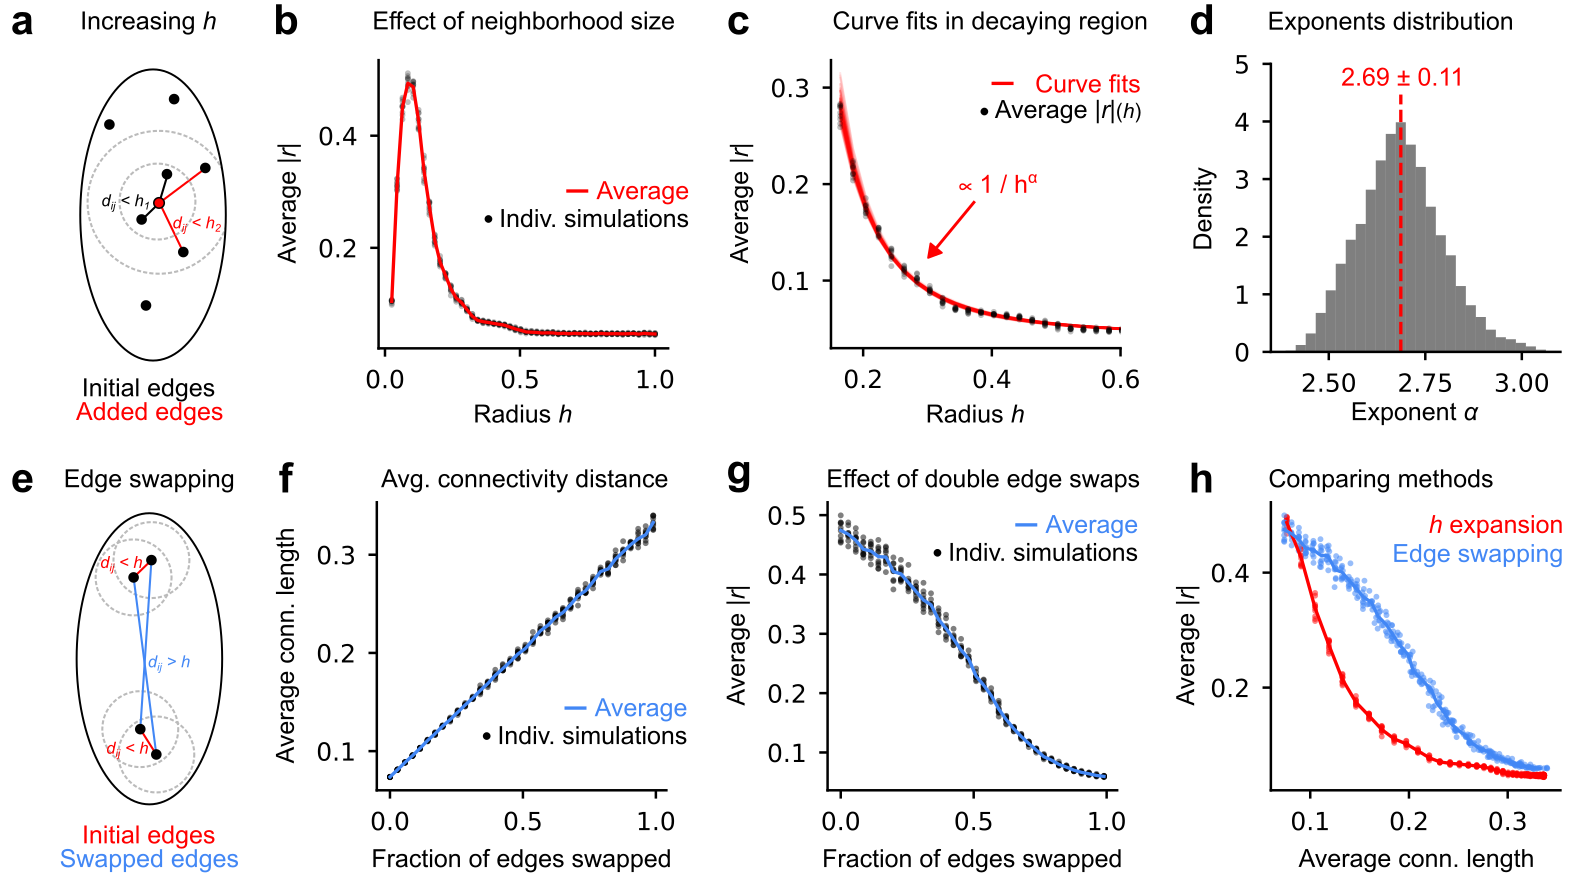
\includegraphics[width=0.95\linewidth]{figures/figure2.png}
    \caption{Geometry-function correspondence decreases as connectivity neighborhood increases. (\textbf{a}) Average absolute Pearson correlation $|r|$ between functional gradients and geometric modes as a function of network size $N$ (computed across the first 50 modes); 10 simulations per $N$ value. (\textbf{b}) Average $|r|$ as a function of connectivity radius $h$; 10 simulations per $h$ value. (\textbf{c}) Power law curve fits in the decaying region of the previous panel; the exponents are estimated from randomly selected individual simulations at each $h$ value. (\textbf{d}) Distribution of fit exponents obtained through bootstrapping and curve fitting individual simulations; a dashed red line indicates the distribution average. (\textbf{e}) Schematization of the double edge swapping procedure; two randomly selected edges (in red) are swapped such that their new lengths (in blue) exceed the initial connectivity radius $h$. (\textbf{f}) Average of connection distances $d$ as a function of the fraction of swapped network edges; $N$ simulations per number of edges swapped. \textbf{g}) Average geometry-function correlation $|r|$ as a function of the fraction of swapped network edges; a gray rectangle indicates a region of linear decrease; 10 simulations per fraction of edges swapped. (\textbf{h}) Comparison of $|r|$ decrease curves as a function of average connectivity distance $d$ achieved through either increasing $h$ (in red) or edge swapping (in blue).}
    \label{fig2}
    \hrulefill
\end{figure*}

\subsection*{Small wavelength eigenmodes progressively disappear as the connectivity radius increases}

The previous analyses demonstrate a loss of geometry-function coupling quantified uniformly across the first 50 gradient-mode pairs. We subsequently investigated the effects of increasing $h$ or swapping edges on the mapping of individual eigenmodes. By visual inspection, a gradual increase in the node connectivity radius $h$ led to the disappearance of high spatial frequency modes (Fig. \ref{fig3}\textbf{a}, average of 10 simulations per matrix, $N=1500$ neurons). Conversely, the first, lower frequency, modes were resilient to this parameter change. At sufficiently large $h$ values, only the first geometric mode mapping persisted (Fig. \ref{fig3}\textbf{a}, right). To more appropriately visualize the effect of $h$ on individual eigenmodes, we plotted the mode correlation matrix diagonals at varying connectivity radii (Fig. \ref{fig3}\textbf{b}). Red arrows roughly denote where individual modes or eigengroups (modes of similar wavelengths) appear to be abruptly cut off by a further increase in $h$ (Fig. \ref{fig3}\textbf{b}). The presence of cutoff points suggests that each geometric gradient exists only under a certain connectivity radius threshold. To quantify this, we estimated the cutoff points of each of the first 50 mode pairs by identifying the $h$ value corresponding to the absolute maximal negative slope of $|r_i|(h)$ (rows of Fig. \ref{fig2}\textbf{b}, Methods). We then compared these cutoff points to the approximate wavelengths $\lambda_i$ of each eigenmode (estimated from geometric mode variograms, Supp. Fig. \ref{supp_variograms}, Methods), observing a strong linear relationship (Fig. \ref{fig3}\textbf{c}, $R^2=0.964$). Thus, the spatial extent of neuronal connections sets a fundamental resolution limit on the eigenmodes that can be expressed within connectivity gradients.

We conducted a similar analysis for simulated networks which instead underwent a double edge swapping procedure to introduce potential long-range connections. In this case, increasing the fraction of swapped edges $\rho_{\text{swaps}}$ led to a smoother and evenly distributed decrease of individual mode mappings, with complete matrix diagonals still visible beyond $\rho_{\text{swaps}}>0.2$ (Fig. \ref{fig3}\textbf{d}). We plotted the mode correlation matrix diagonals against varying $\rho_{\text{swaps}}$ (Fig. \ref{fig3}\textbf{e}), highlighting no clear cutoff points beyond which individual modes seemed to abruptly disappear. Rather, each gradient-mode pair underwent a linear decrease of its correlation $|r|$ with $\rho_{\text{swaps}}$ instead of the plateau-then-zero behavior observed in Fig. \ref{fig3}\textbf{b}. As a consequence, there was no clear relationship observed between maximal slope cutoff points and mode wavelengths (Fig. \ref{fig3}\textbf{f}, $R^2=0.391$). These results suggest that edge swapping leads to a gradual distortion of all geometric gradients, simultaneously, rather than the abrupt disappearance of individual eigenmodes. The different effects of $h$ expansion and edge swapping can be more aptly compared visually in Fig. \ref{fig3}\textbf{g}-\textbf{i}, where the individual mode correlation profiles for varying $h$ are horizontally aligned, relative to their cutoff points. This visualization highlights the abrupt effect of increasing the connectivity radius $h$ (Fig. \ref{fig3}\textbf{h}).

Collectively, these results suggest that geometric gradients with higher spatial frequencies (i.e., smaller wavelengths $\lambda_i$) are the first to disappear when connections extend further in space, while long-wavelength gradients remain largely preserved. For a finite and non-negligible value of $h$, the minimal wavelength of preserved geometric gradients approximately follows a linear relationship with the connectivity radius. This result implies that in real neuronal networks, where arborizations extend over space, there should be an observable cutoff point beyond which gradients and eigenmodes no longer correspond.

\subsection*{Spatial filtering artificially induces geometric gradients}

Our numerical experiments so far demonstrate how the correspondence between connectivity gradients and geometric eigenmodes is driven by short-range neuronal connections. A key implication is that any processing step that amplifies local connectivity can bias this relationship. Spatial filtering, a ubiquitous step in MRI preprocessing, blends signals from neighboring voxels, thereby enhancing correlations. A recent study\cite{watson2023connectopic}, spatial filtering was shown to artificially induce smooth spatial gradients in functional MRI data, which could be misidentified as meaningful connectopies\cite{conne}. This bias was accentuated when considering functional gradients at a smaller spatial scale within individual brain regions. 

\begin{figure}[t]
    \centering
    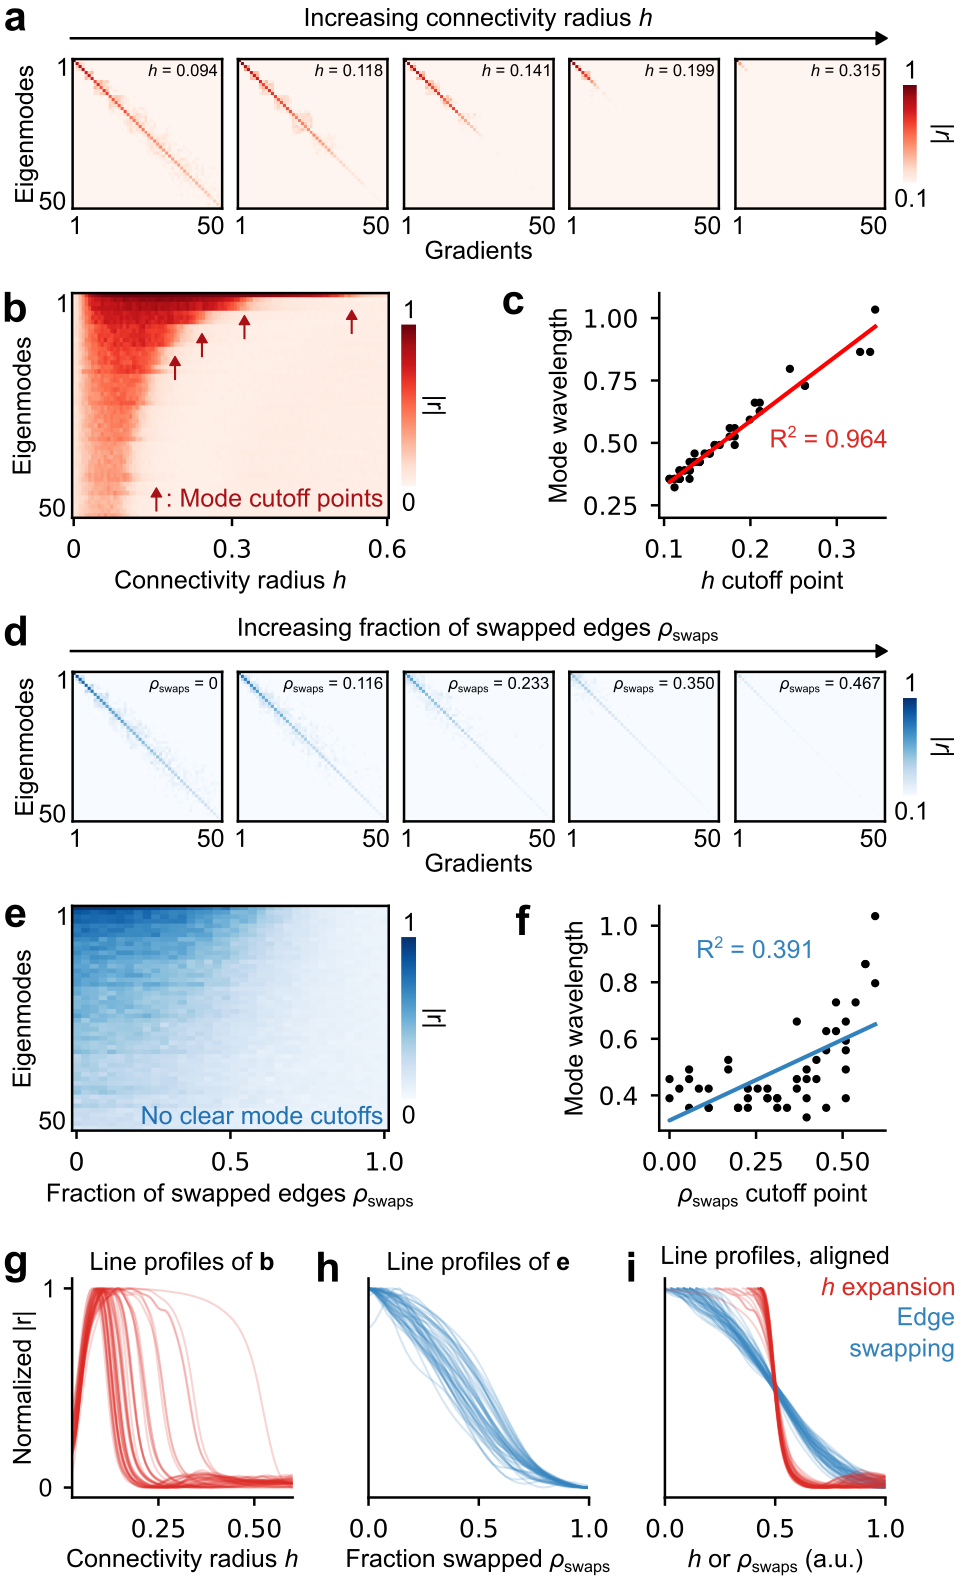
\includegraphics[width=0.5\linewidth]{figures/figure3.png}
    \caption{Degradation of higher spatial frequency modes as connectivity radius increases. (\textbf{a}) Five example mode mapping correlation matrices for increasing connectivity radii $h$; each matrix is averaged across 10 different coordinate ensembles within the ellipsoid ($N=1500$ neurons, 100 averaged simulations per coordinate set). (\textbf{b}) Mode correlation matrix diagonals (columns) for various $h$; arrows denote locations where gradient-mode correlations abruptly drop. (\textbf{c}) Linear relationship between estimated eigenmode wavelengths and the $h$ cutoff points. (\textbf{d}) Five example mode correlation matrices for increasing fractions of swapped network edges $\rho_{\text{swaps}}$; similar averaging parameters as panel \textbf{a}. (\textbf{e}) Mode correlation matrix diagonals (columns) at varying fractions of swapped network edges; notice the absence of abrupt mode decays. (\textbf{f}) Relationship between estimated eigenmode wavelengths and the $\rho_{\text{swaps}}$ cutoff points. (\textbf{g}) Panels \textbf{b} and \textbf{e}, with rows aligned such that cutoff points (defined here as $|r|<0.2$) are centered along the vertical dotted line. (\textbf{h}) Row profiles of the previous panel, highlighting the sharp drop in individual mode correlations observed when increasing $h$, but not edge swapping.}
    \label{fig3}
    \hrulefill
\end{figure}

To evaluate the influence of spatial filtering on geometry-function coupling, we generated "simulations" where neural activity signals were substituted with uncorrelated gaussian noise (Fig. \ref{fig4}\textbf{a}). We spatially filtered the noisy signals using a gaussian spatial kernel (Fig. \ref{fig4}\textbf{b}), combining signals from spatially proximal neurons with a single parameter $\sigma$ dictating the width of the gaussian kernel (Methods). By design, spatial filtering with a small kernel size of $\sigma=0.05$ introduced high artificial correlations between nearby neurons (Fig. \ref{fig4}\textbf{c}). We computed functional gradients from both noisy and filtered correlation matrices, which revealed strikingly smooth gradients in the case where filtering was applied (Fig. \ref{fig4}\textbf{d}). These filtering-induced gradients were strongly correlated with the geometric eigenmodes of the ellipsoid (average $|r|=0.793$ across 20 modes; $|r|=0.604$ across 50 modes; Fig. \ref{fig4}\textbf{e}). This analysis demonstrates how geometric gradients can be artificially driven by spatial filtering, even in the complete absence of correlation between the raw signals. \textcolor{red}{We characterized more generally the effect of various distance-dependent correlation functions, arriving to similar conclusions: matrices generated from monotonously decreasing functions of $d_{ij}$ generally yield geometric gradients (Supp. Fig. X)}.

\begin{figure*}[t]
    \centering
    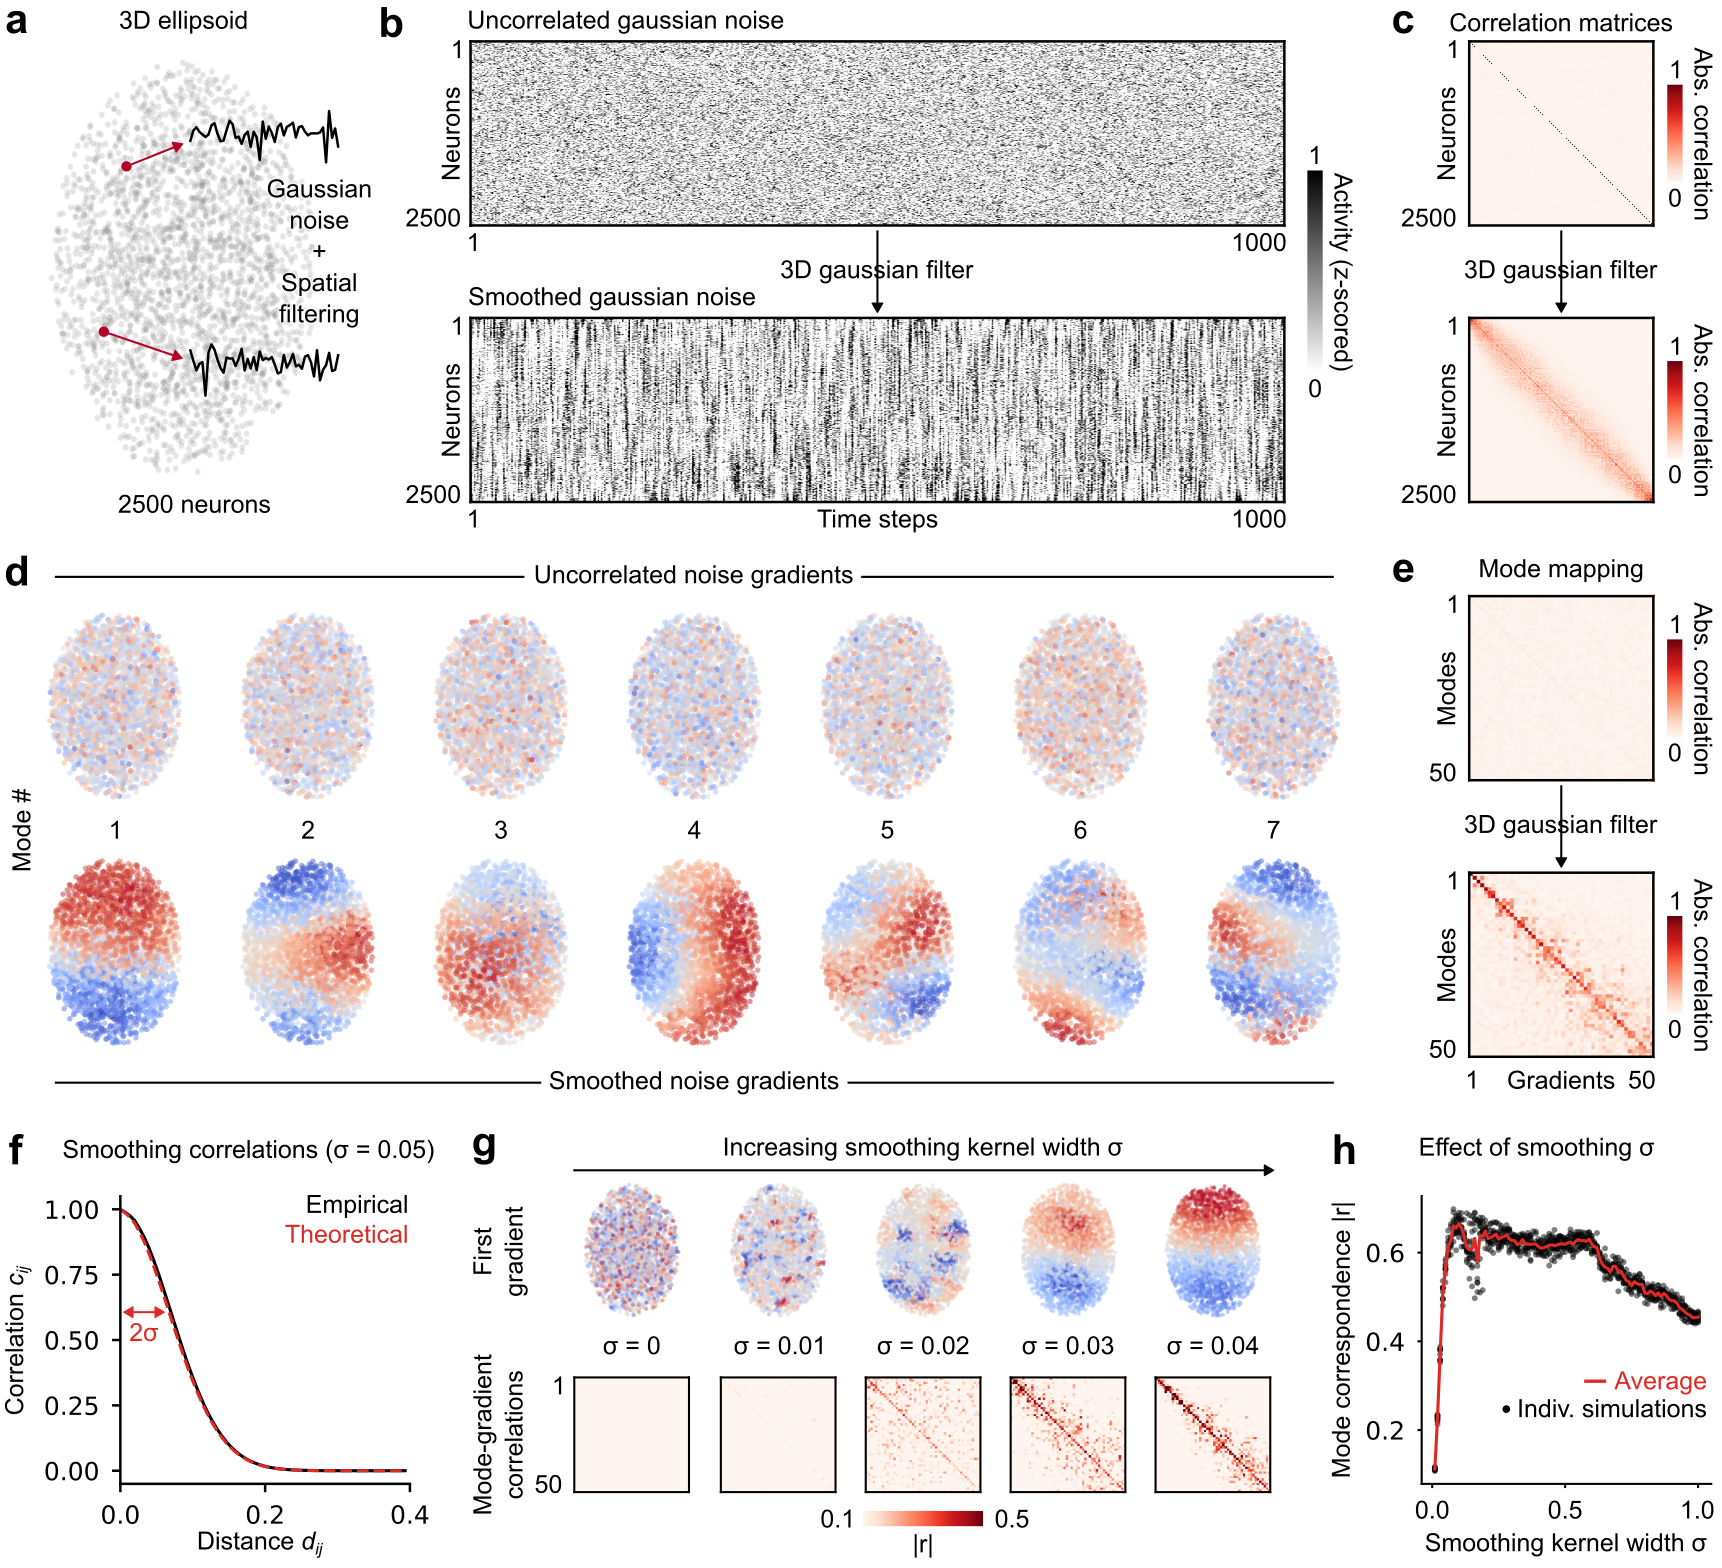
\includegraphics[width=0.95\linewidth]{figures/figure4.png}
    \caption{Spatial filtering of gaussian noise yields geometric functional gradients. (\textbf{a}) Schematization of the "simulations" for the noise filtering analysis; random gaussian noise signals are assigned 3D coordinates within an ellipsoid, then spatially filtered. (\textbf{b}) Top, matrix of random gaussian signals; bottom, same matrix after spatial filtering with $\sigma=0.05$; neurons are ordered along the $z$ axis. (\textbf{c}) Correlation matrix between noisy signals, before (top) and after (bottom) spatial filtering. (\textbf{d}) First 6 functional gradients before (top) and after (bottom) spatial filtering. (\textbf{e}) Correlation matrices of geometric eigenmodes and functional gradients before (top) and after (bottom) spatial filtering. (\textbf{f}) Distributions for theoretical (dashed red line) and empirical (black line) correlations between spatially filtered signals based on the distance $d_{ij}$ between nodes. (\textbf{g}) First functional gradient (top) and mode mapping correlation matrices (bottom) for increasing filtering kernel sizes $\sigma$. (\textbf{h}) Average mode correspondence $|r|$ (first 50 modes/gradients) for varying kernel sizes $\sigma$; black dots correspond to individual simulations (10 per $\sigma$ value, $N=1500$ neurons), while the red curve is the average. Notice a notch at roughly $\sigma=0.2$, which is likely an artifact of numerical discretization.}
    \label{fig4}
    \hrulefill
\end{figure*}

\subsection*{Small filtering kernel sizes strongly drive geometric gradients}

 We next investigated the effect of varying the width of the filtering kernel $\sigma$. First, we mathematically derived the expected filtering-induced correlations $\Tilde{c}_{ij}$ between nodes $i$ and $j$, encapsulated in the simple relationship $\Tilde{c}_{ij}\approx e^{-\nicefrac{d_{ij}^2}{4\sigma^2}}$  where $d_{ij}$ is the distance that separates both nodes (see Supplementary Mathematical Note). This relationship is exact in the limit of an infinite and homogeneous system. Crucially, the width of the filtering-induced correlation gaussian is $2\sigma$, that is, double the initial size of the filtering kernel. We validated numerically that this relationship is correct for small $\sigma=0.05$ relative to the full size of the system, where border effects are more negligible (Fig. \ref{fig4}\textbf{a}, $N=3000$ neurons embedded in 3D ellipsoid). This analysis suggests that the effects of spatial filtering can deceptively induce correlations that extend beyond the spatial footprint of the kernel.

 Further supporting these results, we evaluated the effect of $\sigma$ on the average mode mapping $|r|$, observing the rapid emergence of smooth geometric gradients from very small filtering kernels (Fig. \ref{fig4}\textbf{b}, top). These smooth gradients were strongly correlated with geometric eigenmodes across all 50 mode pairs considered (Fig. \ref{fig4}\textbf{b}, bottom). In Fig. \ref{fig4}\textbf{c}, we plot the average mode correspondence $|r|$ for $\sigma$ ranging from $0$ to $1$, highlighting the very abrupt emergence of geometry with growing $\sigma$ from purely noisy signals. Interestingly, mode correlations remained high and decreased slightly for higher $\sigma$ values that approached the characteristic length of the ellipsoid. This behavior differs from the effect of increasing the connectivity radius $h$, as the geometry-function mapping remains moderate at large kernel sizes. 
 
 These results highlight the high sensitivity of geometric gradients to the effects of spatial filtering, with geometric features emerging from very small filtering kernels, in line with previous reports on the undesirable effects of spatial filtering in MRI studies \cite{watson2023connectopic}. Such findings raise concerns about the potential biases of studying geometric features in imaging modalities where filtering is typically required, especially within smaller brain structures.

\subsection*{Differential effects of combined local connectivity and spatial filtering}

% I commented this out, as the math results will be discussed at the end of the section.

%In this section, we investigate the case where nonzero raw correlations are measured between the signals. In this case, the expected filtered correlations obey
%\begin{align*}
%    \Tilde{c}_{ij} &\approx \frac{\sum_{k, \ell =1}^N e^{\nicefrac{-(d_{ik}^2+d_{j\ell}^2)}{2\sigma^2}}c_{k\ell}}{\sum_{k, \ell=1}^N e^{-\nicefrac{(d_{ik}^2+ d_{i\ell}^2)}{2\sigma^2}}c_{k\ell}},
%\end{align*}
%where the $c_{k\ell}$ are the raw correlations between nodes $k$ and $\ell$ (see Supplementary Material). No further progress can be made without specifying values for the raw correlations. However, figure \ref{supp_dynamics} shows those correlations obey either a gaussian-like or exponential decrease profile. Assuming the real correlations to decrease with distance according to a gaussian curve with variance $\psi^2$, the filtered correlations are given by $\Tilde{c}_{ij}^{\text{Gauss}} \approx e^{\frac{-d_{ij}^2}{2(2\sigma^2+\psi^2)}}$, that is, a gaussian curve whose variance is the sum of the variance of the raw correlations and twice that of the filtering kernel. Note that in the case where no filtering is applied ($\sigma=0$), we obtain the raw correlations, and in the case where no raw correlations are present ($\psi=0$), we obtain the result of the uncorrelated case, as is to be expected.

The previous results consider a simplistic case where there is an absence of correlations between raw neurophysiological signals. This is seldom the case for real data, such as BOLD activity measured in subcortical nuclei. To investigate the potentially nonlinear effects of smoothing an already correlated system, we returned to simulated firing rate dynamics in locally connected networks, and then applied increasing amounts of spatial filtering to neuronal time series (Fig. \ref{fig5}\textbf{a}) before computing pairwise correlations (Fig. \ref{fig5}\textbf{b}). We evaluated the geometry-function coupling for different $(h, \sigma)$ combinations ranging from $h=0.1$ to $h=0.6$, and $\sigma=0$ to $\sigma=0.1$ (Fig. \ref{fig5}\textbf{c}, 10 ellipsoids per parameterization). The different line profiles of the $(h, \sigma)$ grid in Fig. \ref{fig5}\textbf{c} can be visualized in Fig. \ref{fig5}\textbf{d}, where a differential effect of smoothing is observed, depending on the initial value of $h$. In the case where connections are non-local ($h\approx0.6$), the unfiltered geometric mapping is negligible ($|r|<0.1$), but increases steadily as filtering is applied (Fig. \ref{fig5}\textbf{c}, bottom rows; Fig. \ref{fig5}\textbf{c}, bottom curves). When network connections are moderately local ($h\approx0.3$), a partial geometric mapping is initially present. In this case, increasing the filtering kernel width has no effect until a certain kernel size is reached (Fig. \ref{fig5}\textbf{c}, middle rows; Fig. \ref{fig5}\textbf{c}, middle curves). A perhaps counterintuitive effect is observed for the most locally connected systems ($h\approx0.1$), as spatial filtering decreases the initially high geometry-function coupling (Fig. \ref{fig5}\textbf{c}, top rows; Fig. \ref{fig5}\textbf{c}, top curves). Beyond a certain filtering kernel size ($\sigma>0.05$), all systems exhibit monotonically increasing correlations between gradients and eigenmodes, with filtering-induced correlations completely taking over the raw correlations. Taken together, these results highlight the differential and nonlinear effects of spatial filtering on real correlated systems. While geometric gradients may be amplified by excessive spatial filtering, the magnitude of this effect is dependent on the initial locality of connections and correlations within the 3D structure.

\begin{figure*}[t]
    \centering
    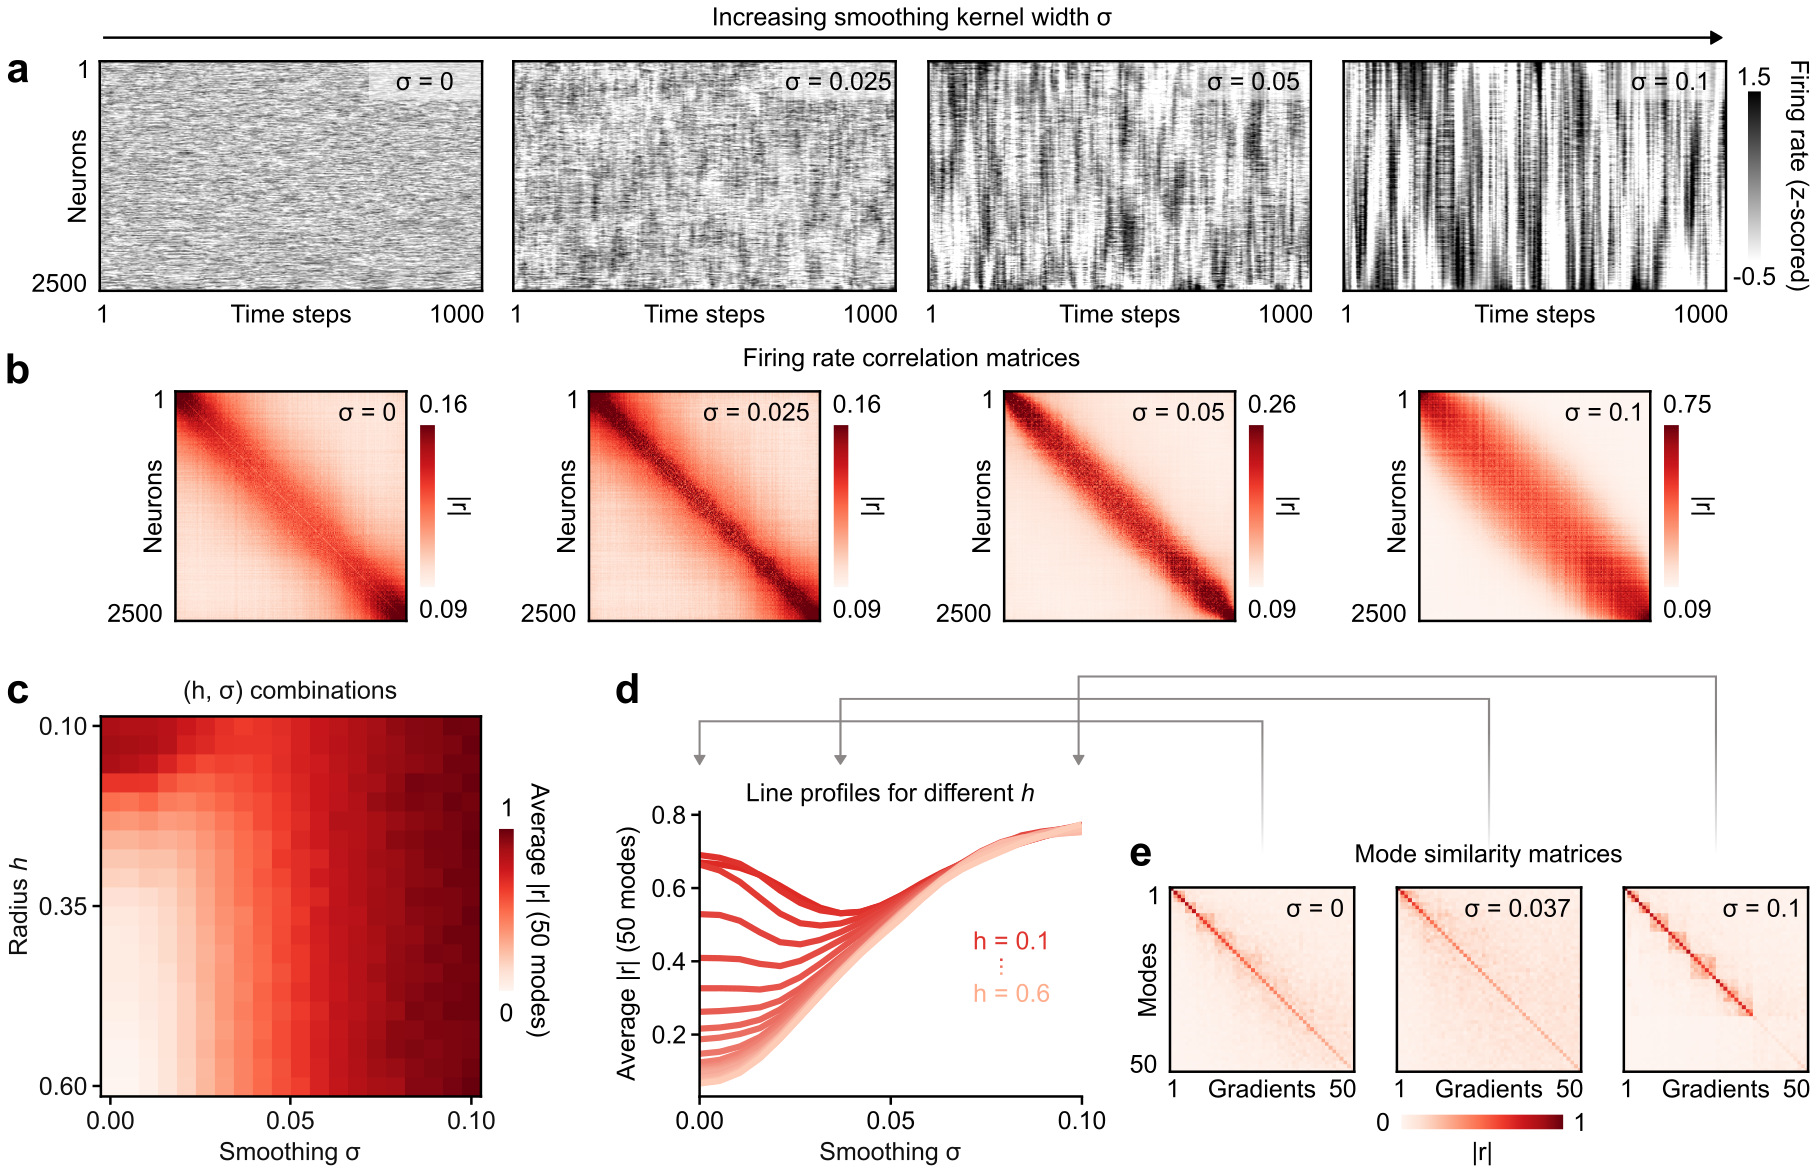
\includegraphics[width=0.95\linewidth]{figures/figure5.png}
    \caption{Differential effects of combined local connectivity and spatial filtering in numerical simulations. (\textbf{a}) Four example simulated firing rate time series for increasing levels of spatial filtering (from left to right); neurons sorted along the $z$ axis of the ellipsoid to accentuate patterns. (\textbf{b}) Pairwise correlations of neuronal firing rates for increasing levels of spatial filtering, corresponding to the four matrices above; colors are scaled to the 5th and 95th percentiles of correlations to improve visualization. (\textbf{c}) Grid of average gradient-eigenmode correlations through 50 modes for different $(h,\sigma)$ parameterizations; $N=1500$ neurons, 10 ellipsoid coordinate sets per pixel, with 100 averaged simulations per set. (\textbf{d}) Row profiles of the previous panel, with mild gaussian filtering applied to the curves for better visualization. (\textbf{e}) Three example mode similarity matrices for $h=0.1$ and three different levels of smoothing; the middle corresponds to the case where smoothing slightly reduces geometric correlations.}
    \label{fig5}
    \hrulefill
\end{figure*}

\subsection*{The larval zebrafish optic tectum exhibits geometric functional gradients}

\begin{figure*}[t]
    \centering
    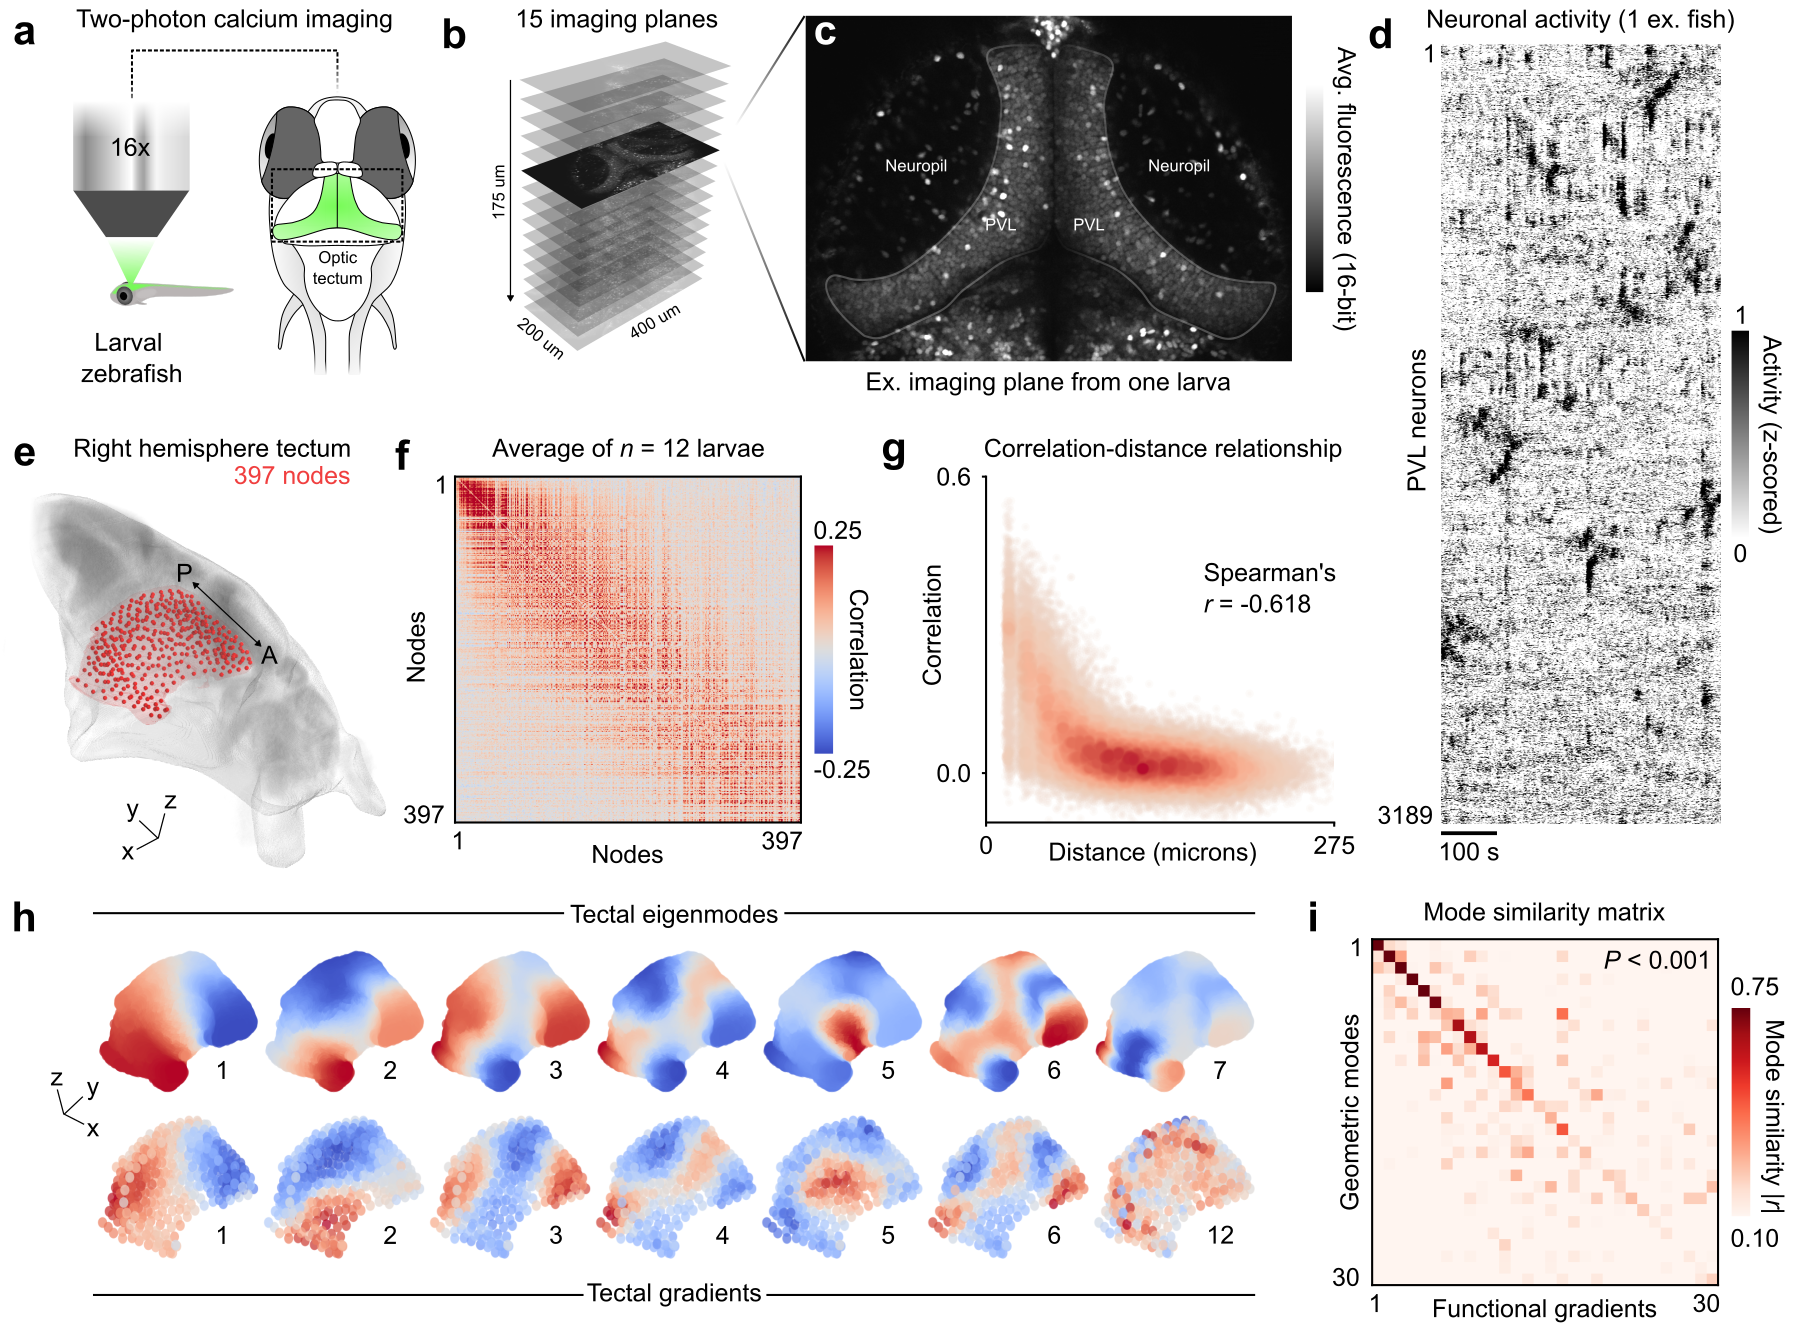
\includegraphics[width=0.95\linewidth]{figures/figure7.png}
    \caption{The larval zebrafish optic tectum exhibits geometric functional gradients. (\textbf{a}) Schematization of the microscopy field of view. (\textbf{b}) Dimensions of the multi-plane imaging volume. (\textbf{c}) One example time-averaged calcium imaging plane, highlighting the nuclear-localized calcium sensor, as well as the periventricular layer (PVL) and neuropil regions of the tectum. (\textbf{d}) Example time series of PVL neurons in the right hemisphere from one animal, sorted using the Rastermap algorithm to accentuate patterns. (\textbf{e}) 3D visualization and anatomical contextualization of the right tectum volume, with tectal nodes used to subdivide the region and allow inter-individual comparisons. (\textbf{f}) Pairwise correlations of node activity, averaged across 12 animals; the matrix is sorted along the antero-posterior brain axis. (\textbf{g}) Correlation-distance relationship obtained from the previous matrix, Spearman's $r=0.618$. (\textbf{h}) Top, first 7 eigenmodes of the right tectum; bottom, corresponding functional gradients derived from calcium activity correlations; red and blue colors represent arbitrary positive and negative values, respectively. (\textbf{i}) Correlation matrix of gradient-eigenmode pairs; notice the diagonal disappearing after roughly 20 modes.}
    \label{fig6}
    \hrulefill
\end{figure*}

Our combined numerical explorations provide three hypotheses that can be readily tested in experimental data. First, if a system is locally connected and correlated, it should exhibit geometric gradients. Second, if arbor sizes are non-negligible, there should be a cutoff point in the gradient-eigenmode mapping. Third, the wavelength of the cutoff eigenmode should reflect the connectivity radius of neurons. To validate these hypotheses, we used volumetric two-photon microscopy to record spontaneous calcium activity in the optic tectum of zebrafish larvae at cellular resolution (Fig. \ref{fig6}\textbf{a}, Tg(\textit{elavl3}:H2B-GCaMP6s)). The optic tectum is the main retinorecipient brain region of the zebrafish and is characterized, in the absence of visual stimulation, by spontaneous bursts of spatially compact neuronal assemblies. This phenomenon is believed to emerge from local recurrent excitatory connections between tectal interneurons.

We recorded 10 minutes of activity from $X\pm Y$ neurons per animal ($n=12$ larvae) distributed throughout the entire tectal volume (15 imaging planes at $\approx2$ Hz, Fig. \ref{fig6}\textbf{b}, Methods). We focused our analysis on cells located within the periventricular layer (PVL neurons, Fig. \ref{fig6}\textbf{c}), which form a continuous and anatomically delineated structure. We also analyzed a single hemisphere to avoid discontinuities in connectivity across the sagittal midplane. Most neurons exhibited low-amplitude calcium fluctuations, with occasional large-amplitude transients involving tens to hundreds of neurons (Fig. \ref{fig6}\textbf{d}, time series sorted using Rastermap; Supp. Video 2). To average correlations across individuals, we used non-rigid registration of anatomical volumes to project all neurons into brain atlas coordinates (mapZebrain atlas, Methods), then subdivided the right hemisphere tectum mask into 400 nodes of roughly equal size (Methods) to which we then assigned individual neurons (Fig. \ref{fig6}\textbf{e}, 397 nodes following exclusion criteria, Methods). We computed nodal time series by averaging single-neuron activity (X $\pm$ Y neurons per node), and then computed the pairwise tectal correlations (Fig. \ref{fig6}\textbf{f}). As expected, we observed a strong decaying profile of group-averaged correlations within the region (Fig. X, Spearman $r=-0.618$), with correlations reaching their baseline level at a distance of roughly $100$ microns. Next, we calculated the functional gradients of group-averaged correlations, as well as the geometric eigenmodes of the brain region's 3-dimensional shape (Methods), and then compared the first 30 gradient-mode pairs to each other. We observed a good correlation between geometry and function across roughly the first 20 modes, beyond which the correspondence vanished (average $|r|=X$ for the first 10 eigenmodes, Fig. \ref{fig6}\textbf{i}). We validated that this mapping was significant by benchmarking against null correlations obtained by spatially shuffling the mode ensembles ($P<0.01$, $1000$ variogram-preserving permutation sets, Methods). We also excluded the possibility that high correlations resulted from the downsampling procedure, as the gradient-eigenmode correlations were nearly identical across varying coarse-graining levels (Supp. Fig. \ref{supp_coarsegraining}\textbf{a}). At the individual level, tectal correlations exhibited variability, resulting in weaker gradient-eigenmode correlations. This is likely due to the limited sampling of individualized correlations resulting from the short duration of each experiment (Supp. Fig. \ref{supp_coarsegraining}\textbf{b}-\textbf{c}).

Together, these results demonstrate that the functional organization of the optic tectum is tightly coupled to its geometry, up to a certain cutoff point where the coupling vanishes, thus validating our first two hypotheses raised by numerical simulations. Most importantly, these findings replicate observations made by Pang, Aquino and colleagues in human subcortical structures, further extending them to a much smaller brain structure at cellular resolution imaging in zebrafish larvae.

\subsection*{Arbor sizes of tectal neurons are consistent with the predicted connectivity radius}

\begin{figure*}[t]
    \centering
    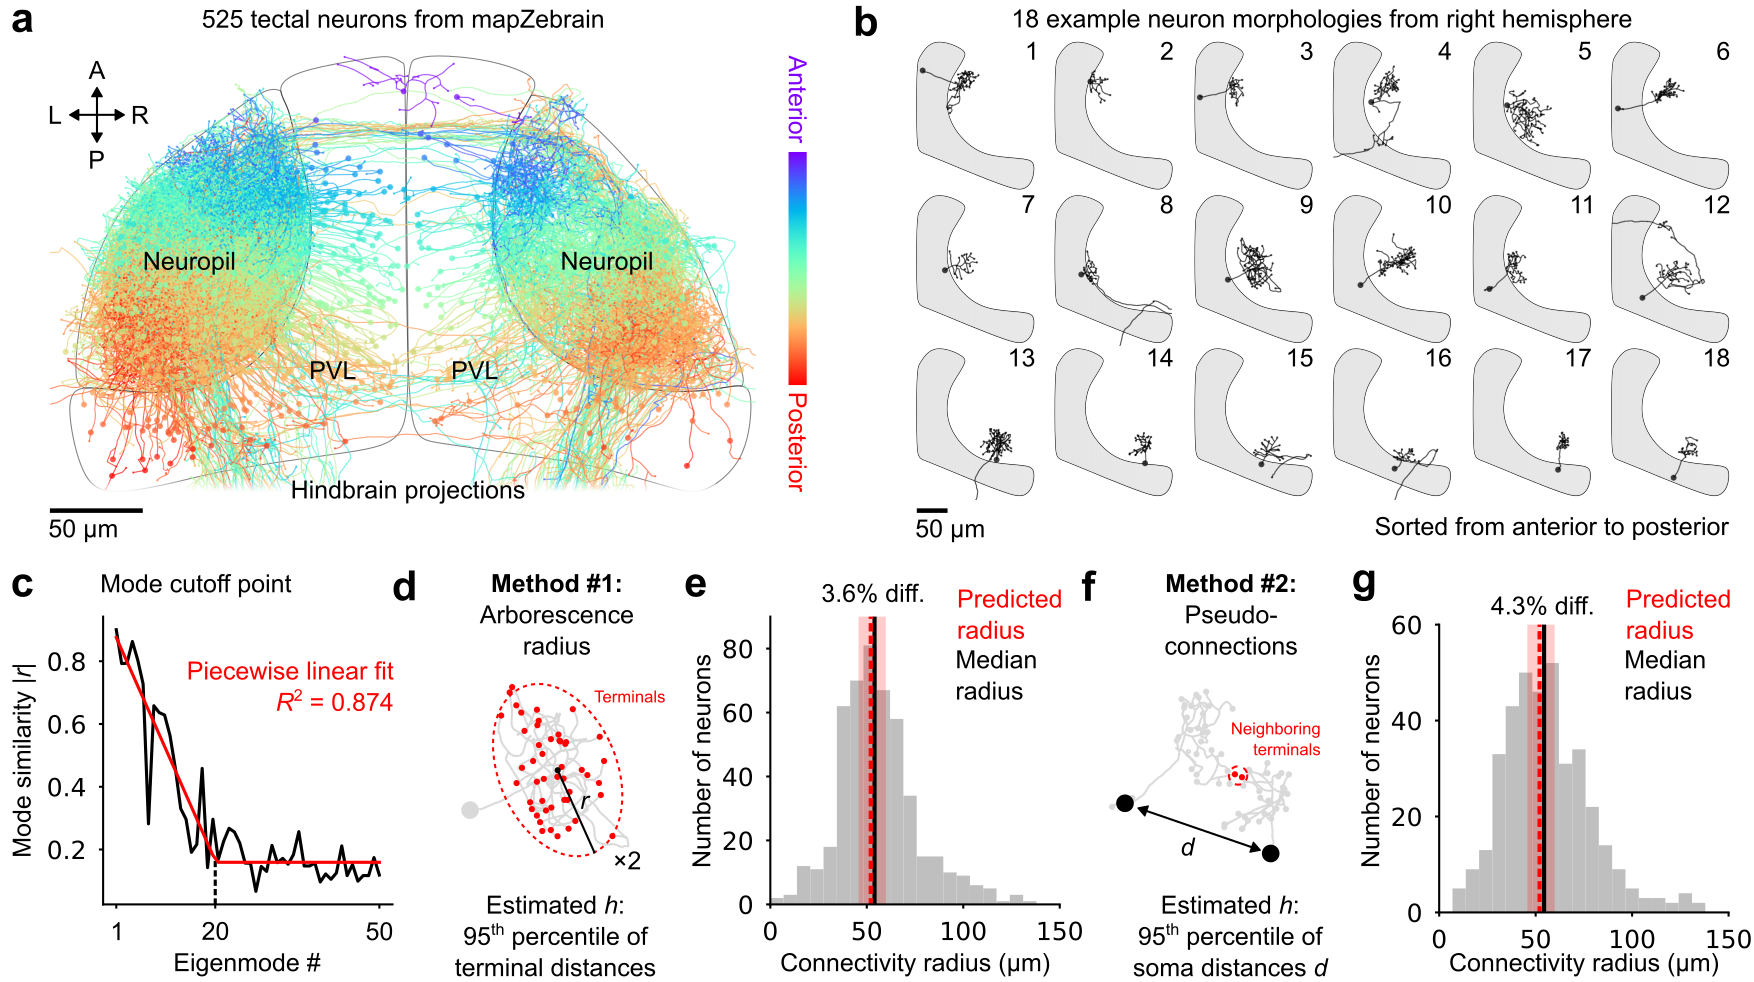
\includegraphics[width=0.95\linewidth]{figures/figure8.png}
    \caption{Arbor sizes of tectal neurons are consistent with the predicted connectivity radius. (\textbf{a}) Top view of 525 tectal neuron morphologies, colored by the antero-posterior location of the cell body, accentuating the topographic organization of neurites within the adjacent neuropil. (\textbf{b}) Example morphologies of 18 neurons, visualized from above. (\textbf{c}) Piecewise-linear regression of tectal gradient-mode correlations to identify a cutoff point, corresponding to eigenmode 20. (\textbf{d}) Schematization of the first connectivity radius estimation method; the Xth percentile of terminal distances (relative to the center of mass) is used to estimate the radius. (\textbf{e}) Distribution of connectivity radii obtained from method 1; the red line indicates the predicted radius from the geometric cutoff point, while the black line is the distribution mean. (\textbf{f}) Schematization of the second connectivity radius estimation method; pseudo-connections are identified from neighboring terminals, then the Xth percentile of soma-soma distances is identified for each neuron. (\textbf{g}) Distribution of connectivity radii obtained from method 2; the red line indicates the predicted radius from the geometric cutoff point, while the black line is the distribution mean.}
    \label{fig7}
    \hrulefill
\end{figure*}

The presence of a cutoff point early in the gradient-eigenmode mapping suggests, based on our simulations, that the connectivity radius of neurons within the region is non negligible, relative to the characteristic length of the system. To characterize the connectivity structure of the optic tectum, we used a single-neuron morphological dataset from the mapZebrain atlas to characterize the arborescence of 525 independently reconstructed tectal neurons (Fig. \ref{fig7}\textbf{a}). Rather than extending neurites radially around the cell body (as in our simple numerical simulations), tectal interneurons project both dendritic and axonal processes into an adjacent neuropil region (Fig. \textbf{a}). While a few neurons innervate the contralateral tectum or downstream hindbrain motor regions, many arbors are entirely contained within the tectal neuropil (Fig. \ref{fig7}\textbf{b}, 18 example morphologies, top view). 

We first identified the cutoff eigenmode from the diagonal of the mode correlation matrix (Fig. \ref{fig6}\textbf{i}) by fitting a piece-wise linear regression with a variable elbow point (Fig. \ref{fig7}\textbf{c}, $R^2=0.874$). While this method differs from the one used previously in Fig. \ref{fig3}, we validated its ability to recover the connectivity radius $h$ from network simulations conducted in tectal geometry ($R^2=0.955$ between cutoff wavelengths inferred from matrix diagonals and connectivity radius $h$, Supp. Fig. \ref{supp_tectum_cutoff}). The estimated cutoff point was eigenmode 20, whose spatial wavelength of $\lambda=150$ microns predicts a connectivity radius of 50 microns between tectal neurons, based on the linear relationship established in Supp. Fig. \ref{supp_tectum_cutoff}. 

To validate this prediction, we analyzed neuron morphologies in two different ways. First, we estimated the diameter of tectal arbors from neurite terminals contained within the tectum neuropil (Methods), then multiplied these diameters by 2 to yield a distribution of estimated connectivity radii (Fig. \ref{fig7}\textbf{d}). This simple method uses overlap between "neurite clouds" to estimate plausible connections. The mean of the connectivity radii distribution was $X$, corresponding to a $X\%$ difference with the estimated radius of $X$. For the second method, we identified pseudo-connections between neurons by finding pairs of cells with at least one pair of terminals separated by less than 5 microns (Fig. \ref{fig7}\textbf{f}, Methods). Then, we estimated the connectivity radius as a certain distance percentile of pseudo-connected cell for each neuron, yielding a distribution of mean $X$ microns, corresponding to a $X\%$ difference with the estimated radius. This second method better accounts for the geometry of tectal neuron arbors, such as their tendency to perpendicularly innervate different layers of the neuropil. In experimental conditions, a cutoff point could also reflect noise in the functional gradients, however we validated that the inferred cutoff point does not vary significantly across a wide range of noise levels in neuronal activity signals (up to 3 data standard deviations in additive noise, Supp. Fig. \ref{supp_noise}). Therefore, it is likely that this cutoff point reflects intrinsic connectivity within the tectum.

Overall, both methods yielded connectivity radii that were, on average, close to the connectivity radius predicted from geometric eigenmodes. These results thus integrate both functional and structural data to verify our third hypothesis: the geometric cutoff point reflects the spatial extent of connectivity.

\subsection*{Whole-brain functional connectivity gradients do not reflect geometry}

Lastly, we considered the effect of spatial filtering on geometric gradients in real data. We used a previous whole-brain two-photon calcium imaging dataset to compute whole-brain functional connectivity gradients (Methods). Brain-wide structural connectivity is heterogeneous, with many long-range projections between regions. We therefore expected a poor geometric coupling in absence of any filtering. We first mapped individual neurons into 987 sub-regions (nodes) of roughly equal size per brain hemisphere, then averaged single-neuron calcium fluorescence within each node before computing pairwise correlations and averaging across both hemispheres and animals (Methods). In parallel, we segmented the brain's 3D external boundaries to delimit a volume for eigenmode calculation, therefore treating the brain as a single homogeneous structure and disregarding potential anatomical boundaries between morphological segments. We computed both single-hemisphere and bi-hemispheric eigenmodes, and then correlated them with single-hemisphere functional gradients, observing virtually no correlation (Supp. Fix. X, $P=X$, 1000 variogram-preserving spatial permutations, Methods). Then, we applied spatial filtering to either single-neuron or node time series, gradually increasing the width of the gaussian kernel. This procedure immediately increased the correlation with geometric eigenmodes, as was the case in our simulations for a non-locally connected system (Fig. \ref{fig5}\textbf{c}-\textbf{d}). In contrast, a spatial filter applied to the tectal data initially had no effect on the geometric mapping, before eventually increasing the correlations (Supp. Fig. X), similar to the case of a moderately local system in our simulations (Fig. \ref{fig5}\textbf{c}-\textbf{d}). Overall, these analyses highlight how spatial filters can make geometric gradients appear out of thin air in real data. However, this effect is less pronounced when the data exhibits real local correlations.

\section*{Discussion}

% Discuss which structures should exhibit geometric gradients
% and why deviations from the geometric regime are interesting
% (for instance, cortical eigenmodes do not reflect gradients, which could indicate
% that widespread coactivation patterns could take over the local correlations)

The influence of space and geometry on nervous system organization is well established, with short-range connections dominating both small and large nervous systems. These local connections support key dynamical phenomena like wave propagation and, under certain approximations, exert a disproportionately large effect compared to long-range ones, enabling a mathematical treatment of the brain as a homogeneous wave-propagating system. Despite the simplicity of this approach, recent studies show that geometrically derived eigenmodes---grounded in the assumption of strong local connectivity---offer a parsimonious basis for decomposing brain activity. This suggests that neural dynamics are shaped by geometry in ways not fully captured by classical connectivity measures.

Here, we used numerical models of neuronal activity across various geometries to explore the mechanisms driving geometric features in brain activity statistics. Specifically, we investigated recent findings from Pang, Aquino, and colleagues, who reported striking similarities between 3D connectivity gradients and geometric eigenmodes in human subcortical structures. To replicate this convergence in different geometries, we imposed a singular constraint on simulations: that neurons are connected to all their neighbors within a certain radius. Regardless of the dynamical model or spatial embedding, the resulting dynamics exhibited local correlations, yielding connectivity gradients that strongly resembled geometric eigenmodes. This outcome aligns with previous theoretical predictions: as network connections become increasingly local, geometry imprints itself onto the network’s structure. Consequently, eigenvectors of the graph Laplacian, a measure of random diffusion akin to connectivity gradients, converge toward those of the LBO derived from the graph's manifold. Despite slight mathematical differences, we observed a similar spectral convergence across multiple gradient derivation methodologies. Further work is needed to clarify relationships between these graph-based measures, but our findings suggest that geometric gradients in 3D connectivity data emerge readily when local connections and correlations are dominant features.

A key implication of our findings is that geometric gradients do not arise solely from wave propagation, as they persist across diverse dynamical systems that do not explicitly implement waves. However, wave-like dynamics are expected to yield geometric gradients due to the local correlations they induce. The observations by Pang, Aquino, and colleagues in subcortical regions likely reflect highly localized activity, but it remains unclear whether cortical waves also manifest in small subcortical nuclei. Recent work combining widefield cortical imaging and Neuropixels recordings in mice shows that cortical waves can be predicted from subcortical activity, which could point toward different mechanisms. Either cortical waves topographically drive subcortical activity, or subcortical regions help coordinate wave propagation, or both. Whether these nuclei inherently support wave-like dynamics, independent of cortical activity, also remains an open question. Resolving subcortical activity with fMRI presents challenges, including low signal-to-noise ratios and susceptibility to motion artifacts due to the small size of these structures. Our results show that spatial filtering, which introduces local correlations, can drive geometric eigenmodes in initially uncorrelated systems, raising concerns about previous fMRI-based findings. However, in systems with inherent local connectivity---which is likely the case for subcortical regions---small filtering kernels had little to no impact on geometric gradients and, in some cases, even degraded them. This suggests that filtering and interpolation may affect gradient analyses differently depending on the underlying connectivity structure. Further work is needed to clarify these effects, particularly in regions like the hippocampus, thalamus, and striatum, which could possibly exhibit geometric features due to their connectivity patterns.

An important aspect of our numerical results is the robustness of geometric gradients to heterogeneities and long-range connections. While real neuronal networks deviate from idealized random geometric models, geometric gradients persist, albeit with slight deterioration, even when 10–20\% of connections are randomized, making this phenomenon biologically plausible. Theoretically, a perfect mapping between gradients and geometric eigenmodes holds only for infinitesimally local connections. However, real neurons have spatially extended arbors that reach beyond their immediate neighbors, causing this mapping to break beyond a specific eigenmode wavelength that reflects the size of underlying arbors, as shown in our simulations. We validated this prediction using two-photon imaging in the larval zebrafish optic tectum, identifying a geometric cutoff point that quantitatively matched neuronal morphologies. While the optic tectum is not entirely homogeneous---featuring local connectivity variations and a layered cell-type organization---its connections remain predominantly local, reflecting the retinotopic arrangement of tectal neurons. The well-documented compact bursting phenomenon in this region produces exponentially decaying correlations, which naturally yield geometric gradients. These results extend the findings of Pang, Aquino, and colleagues to a small vertebrate brain structure at cellular resolution, where activity signals are well-resolved and non-overlapping, and spatial filtering is not necessary.

Despite this empirical validation, our work lacks a formal theoretical framework linking network dynamics to geometric gradients, or arbor sizes to cutoff mode wavelengths, relying instead on a linear estimate of connectivity radius derived from simulations. Further theoretical work is needed to clarify how geometry constrains structural connections (through factors such as physicality and wiring cost minimization) and, in turn, how connections drive geometric features in neuronal dynamics. From this perspective, understanding how geometry shapes brain function is fundamentally tied to the structure-function relationship of brain networks. Beyond synaptic connections, other mechanisms such as extracellular neurotransmitter diffusion and gap junction-mediated synchronization also contribute to localized network dynamics. Exploring these alternative signaling mechanisms could offer deeper insights into the factors influencing geometry-function coupling in brain networks.

Brain morphology varies across mammalian species, neurodevelopmental stages, and is altered in several neurological disorders. Understanding how brain geometry shapes neuronal activity is therefore of both fundamental and clinical interest. Our findings reinforce the central role of short-range connections---an already well-established property of brain networks---as primary drivers of geometric features in three-dimensional brain structures. Given their sensitivity to the heterogeneity and spatial extent of network connections, geometric gradients may serve as a novel, albeit quite indirect functional readout of microcircuit integrity. The increased availability of wiring diagrams at synaptic resolution provides an unprecedented look at the intricate detail of neuronal networks, and indirectly, insights on how they achieve specific computations. An open question remains: do large-scale phenomena like wave propagation emerge as the spatial unfolding of neural computations through precisely arranged microcircuits, or are they merely epiphenomena resulting from simple architectural principles? Resolving this will be key to understanding brain networks across scales.

\section*{Methods}

\subsection*{Geometric eigenmodes}

Geometric eigenmodes are the solutions to the Laplace-Beltrami eigenvalue problem defined on a given geometry. Mathematically, they are functions $\phi_k$ that satisfy $\Delta \phi_k=\lambda_k\phi_k$, where $\Delta$ is the Laplace-Beltrami operator, $\lambda_k$ are the corresponding eigenvalues, and $\phi_k$ form an orthonormal basis ordered by increasing spatial frequency. These eigenmodes represent intrinsic spatial harmonics of the domain and are commonly used to model patterns of diffusion or vibration constrained by geometry. To derive the geometric eigenmodes of each geometry, we first generated volumetric tetrahedral mesh representations using the pygalmesh Python package. This process yielded approximately 30,000–40,000 tetrahedron vertices uniformly distributed throughout each volume and bounded within a unit cube ($x\in[0,1]$), such that a distance of 1 represents a characteristic length scale common to all geometries considered. We then computed the geometric eigenmodes using a finite elements method (FEM) implemented in the LaPy package, solving for the first 100 eigenfunctions of the Laplace-Beltrami operator for each mesh, excluding the first constant eigenmode. The resulting eigenmodes are spatial functions defined over the mesh vertices, ordered by their eigenvalues (spatial wavelengths), with the first mode corresponding to the smoothest pattern (longest wavelength) and higher-order modes representing increasingly fine-grained spatial variations (smallest wavelength).

\subsection*{Simulations of neuronal activity}

We simulated various dynamical models of neurons (described in the following section) embedded within 3D geometries. Although each model involved different parameters, all simulations followed a similar standardized protocol. Neuron coordinates were first randomly sampled from the set of vertices generated during the tetrahedral mesh construction described earlier. A binary connectivity matrix $W^{\text{bin}}$ was then generated by connecting nearby neurons such that $W^{\text{bin}}_{ij}=1$ if $d_{ij} < h$ and $W^{\text{bin}}_{ij}=0$ if $d_{ij} \geq h$, where $h$ is the connectivity radius parameters and $d_{ij}$ is the euclidean distance that separates neurons $i$ and $j$. Note that this binary network definition corresponds to a random geometric network model (cite). Next, $W^{\text{bin}}$ was transformed into a directed, weighted matrix $W$ whose nonzero values were drawn from different distributions specific to each dynamical model, ensuring dynamical stability and rich chaotic dynamics. Neuronal firing rates were then generated by numerically integrating the system over $T=250$ to $1000$ time steps using Euler's method. To quantify emergent functional relationships between neurons, an average correlation matrix $C$ was generated by averaging the absolute pairwise Pearson correlation coefficients $|r|$ of neuronal firing rates over 100 independent simulations. In each run, the connectivity weights and initial conditions were reinitialized, while the neuron positions---and therefore the binary structure $W^{\text{bin}}$---remained fixed. This ensured a representative sampling of possible dynamics unfolding on the same geometric scaffold. We used absolute correlations to capture both large positive and negative relationships between neurons, though in practice, the largest-magnitude correlations were predominantly positive and similar results could be achieved without taking the absolute value, either by normalizing or clipping negative values. Finally, the resulting average correlation matrix $C$ was used for subsequent gradient analysis. For some analyses, we repeated the entire simulation protocol 10 times per geometry and parameterization---each time resampling node coordinates, constructing a new connectivity graph, simulating dynamics, and averaging correlations---to reduce bias introduced by the randomized node coordinates and to suppress noise in the geometric mapping. All numerical simulations were implemented in \verb|PyTorch| using \verb|CUDA|, enabling efficient GPU parallelization and substantially accelerating the integration step.

\subsection*{Dynamical models}

\subsubsection*{Model \#1: Chaotic firing rate network}

For the first and main dynamical model used throughout most of the study, we simulated spontaneous firing rate dynamics from the following equations

\begin{align*}
    \tau\frac{d\textbf{x}}{dt}=-\textbf{x} + g\textbf{W}\textbf{r},\\
    \textbf{r}=\tanh{(\textbf{x})},
\end{align*}

where $\textbf{x}(t)$ describes an internal variable for each neuron, analogous to a membrane potential, while $\textbf{r}(t)$ is the firing rate obtained through a nonlinearity $\tanh (\textbf{x})$. The parameter $\tau$ dictates the time constant of neurons, and $g$ is the network coupling strength, which brings the dynamics into a chaotic regime for $g>1$ in the thermodynamic limit \cite{sompolinsky1988chaos}. Connection weights of $W$ were drawn randomly from a normal distribution $\mathcal{N}(0, \frac{1}{\sqrt{N\rho}})$, with positive and negative weights representing excitatory and inhibitory synapses, respectively. The parameter $\rho$ reflects the empirical average connection density, whose exact value fluctuates with node coordinates and connectivity radius $h$ (networks with small $h$ are sparser, and vice-versa). Crucially, the $\rho$ normalization of connection weights ensures that the overall strength of inputs to each neuron remains constant as the connectivity radius $h$ increases, preventing runaway activity in denser network configurations. We used a stronger coupling of $g=3$ to compensate for network sparsity and to ensure rich chaotic activity time series (Fig. \ref{fig1}\textbf{c}). We used a small time constant of $\tau=3$ to produce faster dynamics and reduce the overall integration time required to properly sample the correlations. Initial conditions $\textbf{x}(0)$ were sampled randomly and uniformly in the range $[-1, 1]$ before numerically integrating the system.

\subsubsection*{Model \#2: Chaotic firing rate network + Dale's law}

For the second dynamical model, we adapted the first dynamical model by changing the neuronal activation function and applying Dale's law to the connectivity matrix. Instead of the standard $\textbf{r}=\tanh(\textbf{x})$, which varies between $-1$ and $1$, we used a strictly positive activation function defined in a previous study,

$$
\textbf{r}(\textbf{x})=
\begin{cases}
r_0\tanh(\textbf{x}/r_0) & \text{for } x\leq0\\
(2-r_0)\tanh(\textbf{x}/(2-r_0)) & \text{for } x>0,
\end{cases}
$$

with firing rates ranging $\textbf{r}(t)$ from 0 to 2. The $r_0$ parameter represents a fixed background firing rate, which we set to $r_0=0.1$. Note that for $r_0=1$, this function reduces to the standard $\tanh$ function. In addition to this change in the neuron dynamics, we applied Dale's law, that is, we imposed strictly positive or negative signs on the columns of $W$. This ensures that each neuron's outputs are strictly excitatory or inbibitory, respectively. We used a $1:1$ ratio of excitatory and inhibitory neurons to maintain properly balanced oscillatory dynamics. These combined changes to the network architecture led to qualitatively different activity, with large spatially patterned population fluctuations that were not present in the more chaotic dynamics of model \#1. Despite these differences, both models produced spatially decaying correlations and comparable geometric gradients (Supp. Fig. \ref{supp_dynamics}).

\subsubsection*{Model \#3: Kuramoto-Sakaguchi oscillators}

For the third dynamical model, we used Kuramoto-Sakaguchi coupled oscillators, whose time-varying phases $\theta$ are described by the following equation

$$\tau\frac{d\theta_i}{dt}=\omega_i+ \frac{g}{N}\sum_{j=1}^N W_{ij}\sin(\theta_j - \theta_i - \alpha_{ij}),$$

where $\tau$ is a global time constant, $\omega_i$ is the fundamental frequency of neuron $i$, $W$ is the connectivity matrix, $g$ is a global coupling strength parameter, and $\alpha_{ij}$ represents a phase lag. For this model, the weights $W$ remained binary and strictly positive. The phase lag matrix $\alpha$ was obtained by multiplying the euclidean distance matrix by an arbitrary scaling parameter, which we set to $50$. This distance-dependent phase lag approximates propagation delays and maintains the network in a chaotic regime. We set $g=2000$, $\tau=100$, and we randomly sampled fundamental frequencies according to $\omega \sim \mathcal{N}(2, 0.1)$. Phases were initialized randomly and uniformly in the $[0, 2\pi]$ range. All parameters were chosen to maximize the geometric quality of the gradients through a linear sweep.

\subsubsection*{Model \#4: Binary stochastic neurons}

For the fourth dynamical model, we implemented a simple binary stochastic neuronal network where the population activity vector $\textbf{x}$ is binary, with ones representing active neurons and zeros representing inactive neurons. The dynamics are described by two parameters, $P_a$, the probability of a neuron becoming active for every active presynaptic neuron, and $P_d$, the probability of a neuron becoming inactive spontaneously at each integrator step. For this model, connection weights $W$ remained binary, and Dale's law was applied in a $1:1$ ratio to ensure balanced excitatory and inhibitory interactions. At each time step, inputs from active neurons were summed at postsynaptic neuron, then the resulting integer number of inputs was multiplied by $P_a$ to yield an activation probability, which we clipped in the range $[0, 1]$. Importantly, the nonsaturating summation of inputs implies that for a sufficient number of positive inputs, postsynaptic neurons are guaranteed to become active. We initialized the network with roughly $10\%$ of active neurons, and used $P_a=0.15$ and $P_d=0.5$ to obtain sustained chaotic dynamics.

\subsubsection*{Model \#5: Spiking neurons + calcium dynamics}

For the fifth and final dynamical model, we implemented a network of leaky integrate-and-fire (LIF) neurons\cite{izhikevich2007dynamical} with simplified calcium dynamics. The temporal evolution of the system is described by the following equations

\vspace{-0.25cm}
\setlength{\jot}{4pt} % default is around 6pt
\begin{align*}
V_{E,i}(t+\Delta t) &= V_{E,i}(t)+\Delta t \Big(g_L(E_L-V_{E,i}(t)) + I_{E, i}(t) + g_{EE,i}(t)(E_E - V_{E,i}(t)) + g_{EI,i}(t)(E_I - V_{E,i}(t))\Big), \\
&\quad V_{E,i}(t)<V_{\text{thresh}}, \\
V_{E,i}(t+\Delta t) &= V_{\text{reset}}, \quad V_{E,i}(t)\geq V_{\text{thresh}}, \\
V_{I,i}(t+\Delta t) &= V_{I,i}(t)+\Delta t \Big(g_L(E_L-V_{E,i}(t)) + I_{I, i}(t) + g_{II,i}(t)(E_I - V_{I,i}(t)) + g_{IE,i}(t)(E_E - V_{I,i}(t))\Big), \\
&\quad V_{I,i}(t)<V_{\text{thresh}}, \\
V_{I,i}(t+\Delta t) &= V_{\text{reset}}, \quad V_{I,i}(t)\geq V_{\text{thresh}}, \\
g_{EE,i}(t + \Delta t) &= g_{EE,i}(t)\Big(1-\frac{\Delta t}{\tau}\Big) + \sum_{j=1}^{N_{E}}c_{EE,i,j}\delta_{E,i}(t), \\
g_{EI,i}(t + \Delta t) &= g_{EI,i}(t)\Big(1-\frac{\Delta t}{\tau}\Big) + \sum_{j=1}^{N_{I}}c_{EI,i,j}\delta_{E,i}(t), \\
g_{II,i}(t + \Delta t) &= g_{II,i}(t)\Big(1-\frac{\Delta t}{\tau}\Big) + \sum_{j=1}^{N_{I}}c_{II,i,j}\delta_{I,i}(t), \\
g_{IE,i}(t + \Delta t) &= g_{IE,i}(t)\Big(1-\frac{\Delta t}{\tau}\Big) + \sum_{j=1}^{N_{E}}c_{IE,i,j}\delta_{E,i}(t).
\end{align*}
\vspace{-0.25cm}

$\textbf{V}_{E}(t)$ and $\textbf{V}_{I}(t)$ represent the membrane voltages of excitatory and inhibitory neurons, respectively, while $\textbf{g}_{EE}(t)$, $\textbf{g}_{EI}(t)$, $\textbf{g}_{IE}(t)$ and $\textbf{g}_{II}(t)$ represent the conductances from $E\to E$, $I\to E$, $E\to I$ and $I\to I$ populations, respectively. $\delta_{E,i}(t)$ and $\delta_{I,i}(t)$ are equal to $1$ if excitatory or inhibitory neuron $i$ emit an action potential at time $t$, else they equal 0. Neurons spike once their membrane voltage exceeds a threshold $V_{\text{thresh}}$, upon which the voltage is immediately reset to $V_{\text{reset}}$ the following time step. $I_E$ and $I_I$ are constant inputs delivered to the excitatory and inhibitory populations. $E_L$, $E_E$ and $E_I$ are the leak, excitatory, and inhibitory reverse potentials, and $g_L$ is the leak conductance. Finally, $\tau$ is the synaptic time constant, and $\Delta t$ is the integrator time step. To simulate the model, we distributed excitatory and inhibitory neurons uniformly throughout the volume, connected them with binary synaptic weights, then used the following set of parameters to generate sustained chaotic dynamics: $g_L=0.15$, $E_L=-75$, $E_E=-40$, $E_I=-90$, $V_{\text{thresh}}=-55$, $V_{\text{reset}}=-75$, $\tau=0.1$, $I_E=5$, $I_I=0$, and $\Delta t=0.025$.

\subsection*{Connectivity gradients}

Connectivity gradients are low-dimensional representations of the large-scale organization of a network, revealing smooth axes of variation in connectivity patterns. When applied to brain data, they capture how neural units are functionally or structurally organized along continuous topographies. Nodes with similar values along specific gradients tend to exhibit similar connectivity patterns, whereas dissimilar nodes are topologically distant along the network's structure. Connectivity gradients were calculated using the diffusion maps algorithm \cite{Coifman2006}. This standard approach consists of calculating the eigendecomposition of a diffusion operator $P_\alpha$ depending on a parameter $\alpha \in [0, 1]$, and defined as 
\begin{align*}
    P_\alpha &= D_\alpha^{-1}W_{\alpha},
\end{align*}
with $W_{\alpha} = D^{-\alpha} C D^{-\alpha}$, $C$ being the connectivity matrix under study (firing rate correlations) and $D$ its degree matrix, that is, the diagonal matrix whose entries are the degrees of $C$, $D_{i i} = \sum_{j}C_{ij}$. The matrix $D_\alpha$ is the degree matrix of $W_\alpha$. The connectivity gradients $G$ are then simply the eigenvectors $\psi_i$ of the diffusion operator $P_\alpha$ scaled by their eigenvalues, $G_i=\lambda_i^t\psi_i$, where $t$ is the diffusion time. The value of $\alpha$ dictates how strongly the density of the sample points (or nodes if C is derived from a graph) on the underlying manifold is taken into account when computing the gradients. Importantly, for specific values of $\alpha$, this family of operators reduces to known diffusion operators. For $\alpha = 1$, $P_\alpha$ simply approximates the Laplace-Beltrami operator on the manifold, removing all influence of the density. For $\alpha = \nicefrac{1}{2}$, $P_\alpha$ approximates Fokker-Planck diffusion. Finally, for $\alpha = 0$, $P_\alpha$ reduces to the transition matrix for the random walk on $C$, $D^{-1}C$. For most of our analyses, we used $\alpha=0.5$, which is standard in the gradient literature. For numerical calculations, we used the BrainSpace implementation of diffusion maps (cite), which by default sets the diffusion time equal to X, providing a tradeoff between small and long timescales (cite). Note that in this study, gradients are not used to embed nodes. Rather, we correlate them to eigenmodes individually, such that the diffusion time parameter becomes irrelevant.

In Supp. Fig. \ref{supp_methods}, we compared three gradient derivation methods. We first demonstrated that geometric eigenmodes can be obtained across the full range of the $\alpha$ parameter. As a second alternative method, we computed gradients from a slightly different matrix. Instead of using raw firing rate correlations $C$, we computed the pairwise correlations of connectivity profiles (rows of $C$), then proceeded with the diffusion maps on this resulting matrix. As a third alternative method, we mimicked the connectopic mapping technique (cite) used in Pang et al (cite), where gradients within a brain region reflect similarities in connectivity profiles with other brain regions. To do this, we simulated two separate neuronal populations of size $N$ and $M$, with the first one sending inputs to the second one. Then, we correlated firing rates across the two systems, and computed a $N\times N$ matrix of connectivity profile similarity for nodes in the first system, relative to the second one. We finally used this similarity matrix to compute gradients using diffusion maps. 

\subsection*{Comparing eigenmodes and gradients}

To compare eigenmodes and gradients, we computed their pairwise absolute correlations $|r_{ij}|$ at the level of network nodes, then solved the following linear sum assignment problem $\text{max}\sum C_{ij}X_{ij}$, where $C$ is the absolute mode correlation matrix and $X$ is a boolean matrix where $X_{ij}=1$ if and only if eigenmode $i$ is assigned to gradient $j$. This procedure is analogous to reordering the columns of the mode correlation matrix while maximizing values on the diagonal. We used the scipy implementation (cite), which uses a modified Jonker-Volgenant algorithm (cite). 

\subsection*{Estimating power law exponent}

To estimate the power law exponent of the $|r|(h)$ curve in Fig. \ref{fig2}\textbf{b}, we randomly subsampled individual simulation results (1 per $h$ increment) in the decaying portion of the curve. For each subsample, we fit a $f(x)=\frac{a}{h^\alpha}+b$ function to recover the exponent $\alpha$. The starting point of the curve fit was randomly selected in the range $h\in[0.16, 0.22]$. We repeated this subsampling procedure 10000 times, yielding a distribution of power law exponents which is shown in Fig. \ref{fig2}\textbf{d}. It is important to note that the estimated exponents are biased by the initial rise of the curve, which likely dampens the initial decay and leads to a slight underestimation of $\alpha$.

\subsection*{Double edge swapping procedure}

The goal of double edge swaps was to preserve the node degrees of geometric graphs while randomizing their connections and introducing long-range connectivity. To do so, we began by selecting two edges at random, say $(u_1, u_2)$ and $(v_1, v_2)$. We then swapped those edges, by replacing them with the new edges $(u_1, v_2)$ and $(v_1, u_2)$. The weights of the initial edges were assigned randomly to the new edges to preserve the total weights (and thus the average degree) of the graph. To ensure that the edge swapping procedure monotonically increases the connectivity distance on average, we rejected swaps where any of the new edges would have a length less than the connectivity radius $h$. We repeated this process by selecting two random edges of length smaller than $h$ and swapped them until a certain fraction $\rho_\text{swaps}$ of the network's edges had been swapped.

\subsection*{Identifying geometric mode cutoffs}

We used two different methods to identify geometric cutoff points, that is, the critical values of $h$ beyond which specific gradient-eigenmode pairings disappeared. One method was applied to numerical simulations, while the other was applied to real data. For simulations, we identified the inflexion point in the S-curve profiles visible in Fig. \ref{fig3}\textbf{h}, corresponding to the point where a given eigenmode is abruptly disappearing from connectivity gradients. To do so, for each mode, we computed the value of $\abs{r}$ for each connectivity radius $h$, and determined the interval $[h_0, h_1]$ for which $\abs{r}$ decreases the most, and for which the adjacent intervals also present a decrease in $\abs{r}$. This last condition serves to guarantee that the cutoff point is in the proper region of the curve and to protect against noise effects. The cutoff value of $h$ was then determined as the middle point of the maximally decreasing interval, $\frac{h_0 + h_1}{2}$. Overall, this method treats each eigenmode separately to identify a relationship between the connectivity radius and mode wavelengths.

For experimental data, we did not have the luxury of varying the connectivity radius. Therefore, to identify a cutoff point, we used a continuous piecewise linear fit on the curve of $\abs{r}$ as a function of the eigenmode number, labelled \#, as shown in Fig. \ref{fig7}\textbf{c}. This piecewise linear fit consists of a decreasing linear part, $-a\#+b_1$, and then a constant (horizontal) part, $b_2$. We found the set of paramaters $a$, $b_1$, $b_2$ and $\#_{cutoff}$ that maximizes the $R^2$ of the regression, and identified the rounded optimal $\#_{cutoff}$ as the eigenmode number corresponding to the cutoff point. This approach is applicable to real data, as it can be measured on an individual mode similarity matrix for a fixed underlying connectivity radius. However, the relationship between cutoff points and $h$ values first has to be estimated from numerical simulations where $h$ is varied, as shown in Supp. Fig. \ref{supp_tectum_cutoff}. We emphasize that the mapping between real data and simulations is not exact, but can nevertheless provide a good estimate of the underlying connectivity.

\subsection*{Estimating eigenmode wavelengths}

To estimate the eigenmode wavelengths $\lambda_k$ in arbitrarily shaped geometries, we computed the variogram of each eigenmode $\phi_k$. For each mode, we randomly selected 2500 vertices and calculated the pairwise squared differences of their eigenmode values, $\sigma^2_{ij}=(\phi_i - \phi_j)^2$. These distances were then averaged within 30 spatial distance bins ranging from 0 to 1. This subsampling process was repeated 10 times per eigenmode to generate an average variogram. The half-wavelength of each eigenmode was estimated as the distance $d$ at which the first peak of the variogram occurred, corresponding to the shortest average distance between regions of maximally opposing signs in the spatial function. We multiplied these distances by 2 to recover full approximate wavelengths.

\subsection*{Spatial filtering}

In both simulations and real data, spatial filtering was applied by combining node activity time series according to the following relationship:

$$\Tilde{r}_i(t)=\sum_{j=1}^N e^{-d_{ij}^2/2\sigma^2} \cdot r_j(t), $$

where $r(t)$ are the raw noisy signals, $\sigma$ is the Gaussian kernel width, and $d_{ij}$ is the distance separating neurons $i$ and $j$. This corresponds to a standard Gaussian filter applied to the continuous set of network coordinates.

\subsection*{Animal model}

All microscopy experiments were conducted \textit{in vivo} on 5-7 dpf Tg(\textit{elavl3}:H2B-GCaMP6s) (cite) zebrafish larvae. Larvae were raised in embryo medium (13.7mM NaCl, 0.54mM KCl, 1.0mM MgSO$_{4}$, 1.3mM CaCl$_{2}$, 0.025mM Na$_{2}$HPO$_{4}$, 0.044mM KH$_{2}$PO$_{4}$, 4.2mM NaHCO$_{3}$, pH 7.2 with HCl 12N) at a density of 1 larva per mL in Petri dishes placed in an incubator at 28$^{\text{o}}$C on a 14:10 hour day/night cycle. From 5 dpf onward, the medium was replaced daily and larvae were fed live \textit{Tetrahymena thermophila} CU428.2 (Cornell University). \textit{T. Thermophila} were grown in Petri dishes in sterile SPP medium (2\% proteose peptone, 0.1\% yeast extract, 0.2\%glucose, 33 $\mu$M FeCl$_{3}$, 250 $\mu$g/mL Penicillin/streptomycin, 0.25$\mu$g/mL Amphotericin B) at room temperature and harvested in the stationary phase. They were then washed from their SPP medium using three centrifugation steps (2min at 0.8g each), followed by pellet resuspension in embryo medium. All protocols were approved by the animal care committee of Université Laval.

\subsection*{Two-photon calcium imaging}

Larvae were embedded in 2\% low-melting point agarose (Invitrogen 16520100) in a 30 mm glass bottom petri dish (Mattek P35G-1.0-14-C) and positioned upright for brain imaging using a toothbrush bristle without direct contact with the animal. The preparation was submerged in embryo medium and placed under the microscope for imaging. All imaging experiments were conducted on a Scientifica SliceScope resonant two-photon microscope (SciScan LabView software) equipped with a Spectra Physics Insight X3 tunable laser. Fluorescence was collected using a piezo-driven 16x water-dipping objective (Nikon, 0.8 NA), reflected by a T585lpxr dichroic mirror, and bandpass filtered (505/119nm) before detection with a GaAsP detector. High-resolution anatomical stacks centered on the tectum were first collected across the full depth of the brain ($1024\times494$ pixels, $\approx$200 planes, 2 microns in z-spacing, 24x frame averaging, zoom level $1.1$) using an excitation wavelength of 860 nm, which is near the isosbestic point of the calcium indicator. Following the structural scan, calcium imaging of the tectum was performed at an excitation wavelength of 920 nm. We sampled neuronal activity from 16 imaging planes ($1024\times494$ pixels, zoom level $1.2$, $2$ Hz volume rate) spaced approximately 12 microns apart, and we excluded the first plane due to piezo recoil artifacts induced by the sawtooth scanning pattern. We delimited the imaging volume by positioning the first plane at the top of the brain where labeled nuclei are first encountered, and then positioned the last plane slightly below the tectum. Power measurements after the objective were maintained at 20 mW, and functional imaging experiments lasted 10 minutes under spontaneous conditions with static red light projected on a screen under the larvae. For the whole-brain imaging experiments, we used similar parameters which are detailed in a previous publication (cite). We analyzed the spontaneous portion of these experiments which lasted roughly 10 minutes, again with static red light projected under the larvae.

\subsection*{Data processing}

Calcium imaging planes were corrected for nonrigid lateral motion using the NoRMCorre algorithm (cite), which is implemented in Python within the CaImAn suite (cite). We used a large patch size of $240\times240$ pixels with a $120$ pixel overlap to prevent local registration artifacts. Then, we segmented fluorescent nuclei from the time-averaged calcium imaging frames of each plane using Cellpose 2.0 (cite). To properly detect the densely labeled nuclei, we trained a custom model on 10 different patches containing roughly 100 neurons each using the expert-in-the-loop method. We then extracted fluorescence signals by averaging pixels within each region of interest (ROI), and detrended the signals using a custom method described in a previous study (cite). Briefly, we used a minimum filter to identify the time-varying baseline of each signal (temporal window of $60$s), then normalized the signals by their baselines to obtain relative fluorescence measurements, $\Delta F(t)=(F(t) - F_0(t))/F_0 (t)$, where $F(t)$ is the raw activity trace and $F_0(t)$ is the inferred baseline. To map each neuron in a standardized anatomical coordinate system, we used ANTs registration (cite) to register the anatomical volume acquired at $\lambda=860$ nm to an atlas template brain generated in the same transgenic line (mapZebrain (cite)), using standard alignment parameters (cite). To ensure a proper alignment of the tectal volume within the larger brain volume, we zeroed the reference template values located outside our approximate imaging field of view. We repeated this alignment procedure between the functional and anatomical imaging volumes acquired at $\lambda=920$ nm and $\lambda=860$ nm respectively, then used the antsApplyTransformsToPoints function twice to transfer the 3D coordinates of neurons from functional to anatomical stacks, then from anatomical to atlas coordinates. 

\subsection*{Computing tectal gradients and eigenmodes}

To compute functional connectivity gradients in the optic tectum, we first identified neurons whose transformed coordinates were located within the tectal periventricular layer using a brain region mask defined in the atlas. Then, we subdivided the right hemisphere mask into 400 evenly spaced subregions using k-means clustering, and then assigned individual neurons to their nearest neighboring node. Importantly, neurons were assigned to one node only, thus avoiding the blending of signals between adjacent nodes. We averaged neuronal activity within each node, then correlated these signals to yield anatomically comparable correlation matrices across animals, which we then averaged before computing gradients on the group-average matrix, which exhibited very few negative values. We used absolute correlations to compute gradients, which yielded similar results than thresholded correlations clipped in the range $[0, 1]$ to remove negative values. For gradients computed on individual FC matrices (Supp. Fig. \ref{supp_coarsegraining}\textbf{b}), negative values were more prominent, and we rescaled matrices in the range $[0, 1]$ before computing gradients. For eigenmode calculation, we used the right hemisphere of the 3D PVL binary mask from the brain atlas as a volume for mesh generation. We generated a tetrahedral mesh and solved the eigenmodes using the FEM from LaPy as described earlier.

\subsection*{Morphological analysis}

To estimate the connectivity radius of tectal neurons, we leveraged a dataset of 4327 independently reconstructed neurons from mapZebrain, compiled across different animals (cite). Of these neurons, 525 have their soma located within the periventricular layer (PVL), corresponding to where nuclei are located in our calcium imaging dataset. For each PVL neuron, we identified arbor terminals located within the adjacent tectal neuropil as putative synapses, and then used two different methods to estimate the connectivity radius. For the first method, we measured the center of mass (COM) of terminal coordinates for each neuron. Then, we measured each terminal's distance from the arbor COM, and defined the arbor radius as the 95th percentile of terminal-COM distances. We used a high percentile rather than the maximum distance to capture most of the arbor without including terminals found on distant projections leaving the region (for instance, see neuron 12 in Fig. \ref{fig7}\textbf{b}). This yielded a distribution of arbor radii, which we multiplied by 2 to obtain approximate connectivity radii, that is, hypothetical distances between the soma of two neurons whose arbors barely intersect each other. For the second method, we identified all pairs of pseudo-connected neurons, that is, neurons with terminals located within 5 microns of each other or less. Then, for each neuron, we defined its connectivity radius as the 95th percentile of soma-soma distances with its pseudo-connected partners. Again, we used a high percentile rather than the maximum distance to obtain a representative measure that is less sensitive to outliers. Once compiled across all cells, we used the median values of both radius distributions to compare with the connectivity radius predicted from the geometric cutoff point identified in functional imaging data. While the first method approximates arbors as spherical objects, the second one better accounts for the geometry of arbors, which tend to innervate specific layers of the neuropil. Regardless, both methods yielded very similar distributions.

\subsection*{Computing whole-brain gradients and eigenmodes}

We used a previously published dataset from our lab (cite) to investigate the relationship between whole-brain connectivity gradients and geometric eigenmodes. We used a high-resolution parcellation of 987 nodes per brain hemisphere, obtained by fragmenting larger anatomical brain region masks with k-means clustering, to coarse-grain the activity of roughly $55,000$ neurons per animal ($n=22$ larvae). Then, we averaged node time series (the first 10 minutes, which correspond to spontaneous activity) from both hemispheres, computed pairwise correlations between nodes, and averaged individual correlation matrices to generate a group-average FC matrix. We calculated FC gradients using the diffusion maps algorithm on the absolute correlations $|C|$ with $\alpha=0.5$ as per the rest of this study. In parallel, we calculated geometric eigenmodes on a 3D whole-brain mask obtained by manually delimiting the external boundaries of the brain. More specifically, we used a cytosolic GCaMP template to properly visualize cell bodies and neuropil regions and segmented the brain boundaries on each 2D plane. Then, we mirrored the segmentations, applied 3D smoothing, and binarized again to obtain a smooth 3D volume of the brain. We generated a tetrahedral mesh of this volume and calculated eigenmodes similarly as described previously, then mapped the eigenmode values to the brain region nodes using nearest neighbors before finally correlating both mode ensembles after establishing their optimal mapping.

\subsection*{Statistics}

Various statistical tests were used throughout the study, depending on the nature of the data and the comparisons being made. In each case, the specific test, sample size, and exact $P$-values are reported in the relevant figure legends or text. All tests were two-sided unless otherwise specified, and significance was defined as $P<0.05$. No statistical methods were used to predetermine sample sizes. Spatial permutations were performed using the BrainSMASH toolbox, which randomizes data while approximately preserving its spatial autocorrelation as captured by the variogram.

\section*{Data availability}

Data used within this study are available at X. Raw calcium imaging videos are available upon reasonable request to the authors.

\section*{Code availability}

Code used in this study is available via X and X.






%\printbibliography
\bibliographystyle{unsrt}
\bibliography{article/references}








\section*{Acknowledgements}

We acknowledge Calcul Québec and Digital Research Alliance of Canada for their technical support and computing infrastructures. We are thankful for discussions with members of the Dynamical Research Lab and the PDK Lab.

\section*{Author contributions}

AL and OR designed the study. AL conducted numerical experiments. OR performed mathematical calculations. AL conducted calcium imaging experiments and analyzed the data. AL, OR and AA contributed to code development. AL and OR wrote the initial manuscript. All authors contributed to manuscript revision. PDK, AA, and PD acquired funding and supervised the project.

\section*{Competing interests}

The authors declare no competing interests. 

\newpage



\section*{Supplementary Material}

\subsection*{Calculation of filtering-induced correlations}

In the main text, we claimed that the expected correlations induced by filtering uncorrelated gaussian noise signals are given by
\begin{align*}
    \Tilde{c}_{ij} \approx e^{-d_{ij}^2/4\sigma^2}.
\end{align*}
Here, we give the derivation for this result. Correlations are taken as the Pearson correlation coefficient,  which, for a sample of variables $x$ and $y$ of size $n$, is given by
\begin{align*}
    r_{xy} = \frac{\sum_{i=1}^n(x_i-\bar{x})(y_i-\bar{y})}{\sqrt{\sum ^n _{i=1}(x_i - \bar{x})^2} \sqrt{\sum ^n _{i=1}(y_i - \bar{y})^2}},
\end{align*}
where $\bar{x}$ and $\bar{y}$ are the average values of $x$ and $y$. Since we are interested in the expected value of this coefficient for gaussian random signals, we will instead proceed with our calculations using the following coefficient:
\begin{align}
    c_{ij} &= \frac{\expval{f_if_j}-\expval{f_i}\expval{f_j}}{\sigma_{f_i}\sigma_{f_j}},
    \label{eq:exp_coefficient}
\end{align}
where $f_i$ would be the random variable corresponding to the activity of node $i$ on a observed unknown network, for instance. If we treat those signals as independent and with mean $0$, the expected coefficient is simply
\begin{align*}
    c_{ij} &= \frac{\expval{f_i}\expval{f_j}-\expval{f_i}\expval{f_j}}{\sigma_{f_i}\sigma_{f_j}} = 0.
\end{align*}
Now, we introduce spatial filtering to the signal. This procedure consists of convoluting the signal with a gaussian filter, which yields
\begin{align*}
    \Tilde{f}_i &= \frac{1}{\sqrt{2\pi}\sigma N}\sum_{k=1}^N e^{-\nicefrac{d_{ik}^2}{2\sigma^2}}f_k,
\end{align*}
where $\sigma$ is the standard deviation of the gaussian filter, $N$ is the number of nodes in the network and $d_{ij}$ is the distance between nodes $i$ and $j$. Since all $f_k$ have mean $0$, the filtered signals $\Tilde{f}_i$ also have mean $0$. The covariance between these filtered signals is then
\begin{align*}
    \expval{\Tilde{f}_i\Tilde{f}_j} &= \frac{1}{2\pi\sigma^2N^2}\expval{\qty(\sum_{k=1}^N e^{-\nicefrac{d_{ik}^2}{2\sigma^2}}f_k)\qty(\sum_{\ell=1}^N e^{-\nicefrac{d_{j\ell}^2}{2\sigma^2}}f_\ell)}\\
    &= \frac{1}{2\pi\sigma^2N^2}\sum_{k, \ell =1}^N e^{\nicefrac{-(d_{ik}^2+d_{j\ell}^2)}{2\sigma^2}}\expval{f_kf_\ell}.
\end{align*}
Since the raw signals are independent, $\expval{f_kf_\ell} = \expval{f_k^2}\delta_{k\ell} = \sigma_{f_k}^2\delta_{k\ell}$, with $\delta_{k\ell}$ the Kronecker delta. The covariance is therefore
\begin{align*}
    \expval{\Tilde{f}_i\Tilde{f}_j} &= \frac{1}{2\pi\sigma^2N^2}\sum_{k = 1}^N e^{\nicefrac{-(d_{ik}^2+d_{jk}^2)}{2\sigma^2}}\sigma_{f_k}^2.
\end{align*}
For the standard deviations,
\begin{align*}
    \sigma^2_{\Tilde{f}_i} &= \expval{\Tilde{f}_i^2}\\
    &= \frac{1}{2\pi\sigma^2N^2}\expval{\qty(\sum_{k=1}^N e^{-\nicefrac{d_{ik}^2}{2\sigma^2}}f_k)\qty(\sum_{\ell=1}^N e^{-\nicefrac{d_{i\ell}^2}{2\sigma^2}}f_\ell)}\\
    &= \frac{1}{2\pi\sigma^2N^2}\expval{\sum_{k, \ell =1}^N e^{-(\nicefrac{d_{ik}^2 + d_{i\ell}^2)}{2\sigma^2}}f_kf_\ell}\\
    &= \frac{1}{2\pi\sigma^2N^2}\sum_{k=1}^N e^{-\nicefrac{d_{ik}^2}{\sigma^2}}\sigma_{f_k}^2.
\end{align*}
If all the signals are i.i.d, that is they all have the same variance, then the expected correlation between the filtered signals is
\begin{align}
    \Tilde{c}_{ij} &= \frac{\sum_{k = 1}^N e^{\nicefrac{-(d_{ik}^2+d_{jk}^2)}{2\sigma^2}}}{\sqrt{\qty(\sum_{k=1}^N e^{-\nicefrac{d_{ik}^2}{\sigma^2}})\qty(\sum_{\ell=1}^N e^{-\nicefrac{d_{j\ell}^2}{\sigma^2}})}} > 0.
    \label{eq:artificial_correlation}
\end{align}
Exact computation of the expected value for the filtered correlations depends on the distribution of the distances between the nodes and on the precise geometry of the manifold, which makes that computation impossible in general. However, under the assumption that nodes are distributed uniformly in the manifold, and ignoring the effect of the manifold's boundaries, we can use a continuous approximation which should be exact as $N\to \infty$. Under these assumptions, both sums in the denominator are approximated as
\begin{align*}
    \sum_{k=1}^N e^{-\nicefrac{d_{ik}^2}{\sigma^2}} &\approx \int_0^{2\pi}\int_0^\infty e^{-r^2/\sigma^2}r\dd r\dd\theta\\
    &= \pi\sigma^2.
\end{align*}

Since the choice of node $i$ or $j$ should have no impact on the sum, both sums at the denominator are equal, and as such the denominator as a whole is approximately $\pi\sigma^2$. 

The numerator is harder to estimate, but we can use a similar method, using the law of cosines and the following geometric construction:

\begin{center}
\begin{tikzpicture}

    % Define the center, the point on the circle, and the external point
    \coordinate (i) at (0,0); % Center of the circle
    \coordinate (k) at (1,2); % Point on the circle
    \coordinate (j) at (4,0); % Point outside the circle

    % Draw the circle
    \draw (i) circle[radius=sqrt(5)];

    % Draw the radius
    \draw[dashed] (i) -- (k);

    % Draw the lines from j to i and j to k
    \draw[dashed] (j) -- (i);
    \draw[dashed] (j) -- (k);

    % Draw the center, boundary point, and external point
    \fill (i) circle[radius=2pt];
    \fill (k) circle[radius=2pt];
    \fill (j) circle[radius=2pt];

    % Label the center, boundary point, and external point
    \node at (i) [label=left:$i$] {};
    \node at (k) [label=above:$k$] {};
    \node at (j) [label=above:$j$] {};

    % Label the radius
    \node at ($(i)!0.5!(k)$) [above left] {$r$};

    % Label the lines
    \node at ($(i)!0.4!(j)$) [below right] {$d_{ij}$};
    \node at ($(k)!0.5!(j)$) [above right] {$d_{jk}$};
    \pic [draw, ->, "$\theta$", angle eccentricity=1.5] {angle = j--i--k};
\end{tikzpicture}
\end{center}

With the law of cosines, 
\begin{equation*}
    d_{jk}^2 = r^2+d_{ij}^2-2rd_{ij}\cos\theta.
\end{equation*}
As such, the integral approximating the numerator is
\begin{align*}
    \sum_{k = 1}^N e^{\frac{-(d_{ik}^2+d_{jk}^2)}{2\sigma^2}} &\approx \int_{0}^{2\pi}\int_0^{\infty}e^{-(2r^2+d_{ij}^2-2rd_{ij}\cos\theta)/2\sigma^2}r\dd r\dd \theta\\
    &= e^{\frac{-d_{ij}^2}{2\sigma^2}}\int_0^{\infty}e^{-\nicefrac{r^2}{\sigma^2}}r\dd r\int_{0}^{2\pi}e^{rd_{ij}\cos\theta/\sigma^2}\dd \theta\\
    &= 2\pi e^{\frac{-d_{ij}^2}{2\sigma^2}}\int_0^{\infty}e^{-\nicefrac{r^2}{\sigma^2}}I_0\qty(\frac{d_{ij}r}{\sigma^2})r\dd r\\
    &= 2\pi e^{\frac{-d_{ij}^2}{2\sigma^2}} \sum_{n=0}^\infty \frac{d_{ij}^{2m}}{(2\sigma^2)^{2m} m!^2}\int_0^\infty r^{2m+1} e^{-\frac{r^2}{\sigma^2}} \dd r\\
    &= \pi \sigma^2 e^{\frac{-d_{ij}^2}{2\sigma^2}} \sum_{n=0}^\infty \frac{(d_{ij}^{2})^{m}}{(4\sigma^2)^{m} m!}\\
    &= \pi \sigma^2 e^{\nicefrac{-d_{ij}^2}{4\sigma^2}}.
\end{align*}
Thus,
\begin{align*}
    \Tilde{c}_{ij} \approx e^{-d_{ij}^2/4\sigma^2}.
\end{align*}

In the case where the raw signals have nonzero correlations, 

\begin{align*}
    \Tilde{c}_{ij} &\approx \frac{\sum_{k, \ell =1}^N e^{\nicefrac{-(d_{ik}^2+d_{j\ell}^2)}{2\sigma^2}}c_{k\ell}\sigma_{f_k}\sigma_{f_\ell}}{\sum_{k, \ell=1}^N e^{-\nicefrac{(d_{ik}^2+ d_{i\ell}^2)}{2\sigma^2}}c_{k\ell}\sigma_{f_k}\sigma_{f_\ell}},
\end{align*}
where the $c_{k\ell}$ are the raw correlations between the signals of nodes $k$ and $\ell$. Expecting the variances of the signals to either be $1$ or to approximately cancel out, this simplifies to
\begin{align*}
    \Tilde{c}_{ij} &\approx \frac{\sum_{k, \ell =1}^N e^{\nicefrac{-(d_{ik}^2+d_{j\ell}^2)}{2\sigma^2}}c_{k\ell}}{\sum_{k, \ell=1}^N e^{-\nicefrac{(d_{ik}^2+ d_{i\ell}^2)}{2\sigma^2}}c_{k\ell}}.
\end{align*}
The only correlation profile for which a closed form can be obtained, to our knowledge, is a gaussian correlation profile $c_{k\ell} = e^{-d^2_{k\ell}}/2\psi^2$. In this case, following the same calculation as above, we obtain
\begin{align*}
    \Tilde{c}_{ij} &\approx e^{\frac{-d_{ij}^2}{2}\qty(\frac{1}{2\sigma^2+\psi^2})}.
\end{align*}
Note that for $\psi^2 = 0$, this results returns to the uncorrelated case, and for $\sigma = 0$, we obtain the filtering kernel itself, as is to be expected.

In the case where the raw correlations are decrease exponentially with distance, the calculation does not yield a closed form.

\newpage
%\end{multicols}
\section*{Supplementary figures}

\renewcommand{\thefigure}{S\arabic{figure}}
\addtocounter{figure}{-7}

\begin{figure*}[h]
    \centering
    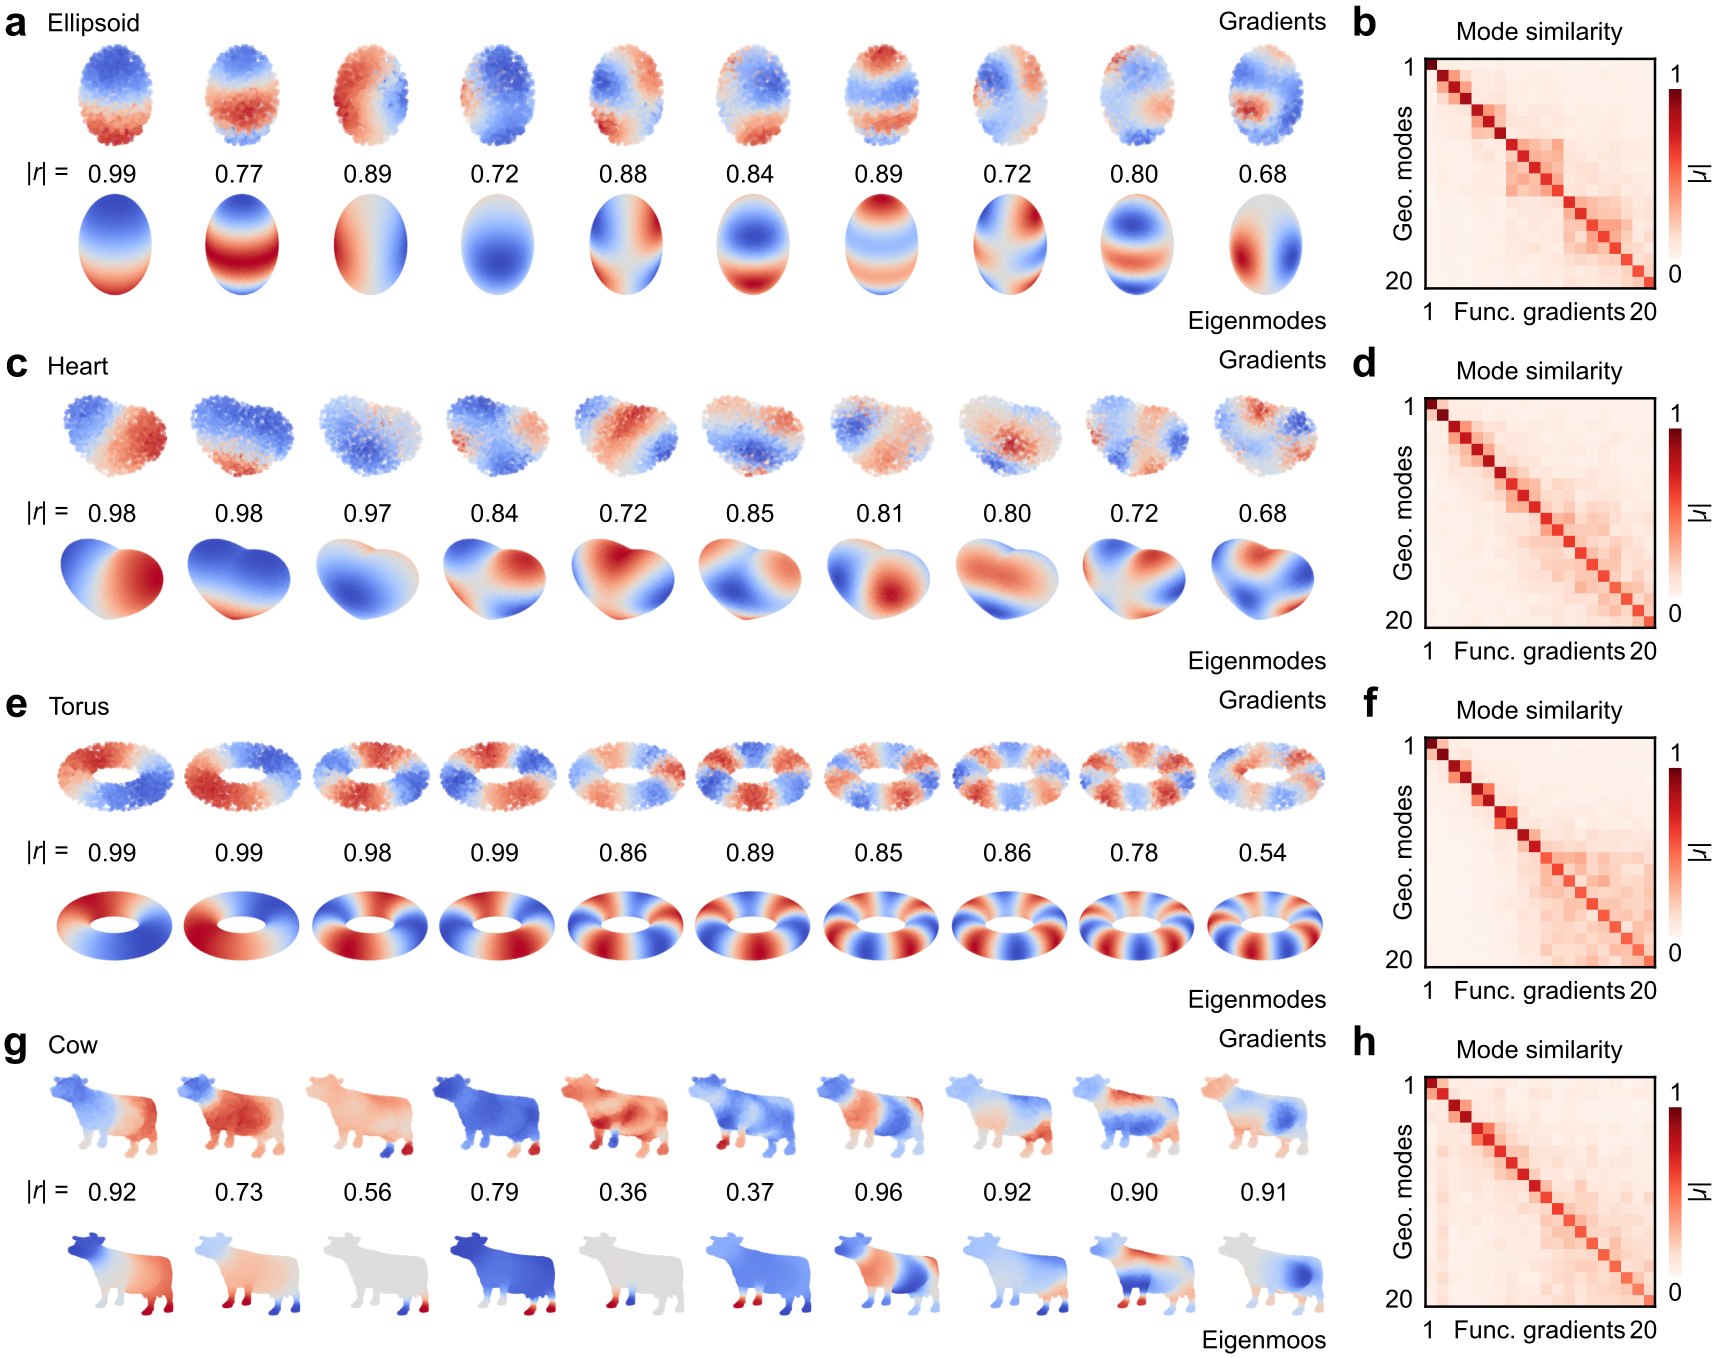
\includegraphics[width=1.0\linewidth]{figures/supp_geometries.png}
    \caption{Comparison of functional connectivity gradients and geometric eigenmodes in various geometries. (\textbf{a}) Gradients and eigenmodes of an ellipsoid shape; absolute correlations $|r|$ are indicated for the first 10 mode pairs (one representative simulation). (\textbf{b}) Gradients-eigenmodes similarity matrix for the ellipsoid geometry, averaged across 10 coordinate sets. (\textbf{c}) Gradients and eigenmodes of a heart shape. (\textbf{d}) Gradients-eigenmodes similarity matrix for the heart geometry, averaged across 10 coordinate sets. (\textbf{e}) Gradients and eigenmodes of a torus shape. (\textbf{f}) Gradients-eigenmodes similarity matrix for the torus geometry, averaged across 10 coordinate sets. (\textbf{g}) Gradients and eigenmodes of a cow shape. (\textbf{h}) Gradients-eigenmodes similarity matrix for the cow geometry, averaged across 10 coordinate sets.}
    \label{supp_geometries}
\end{figure*}

\newpage

\begin{figure*}[t]
    \centering
    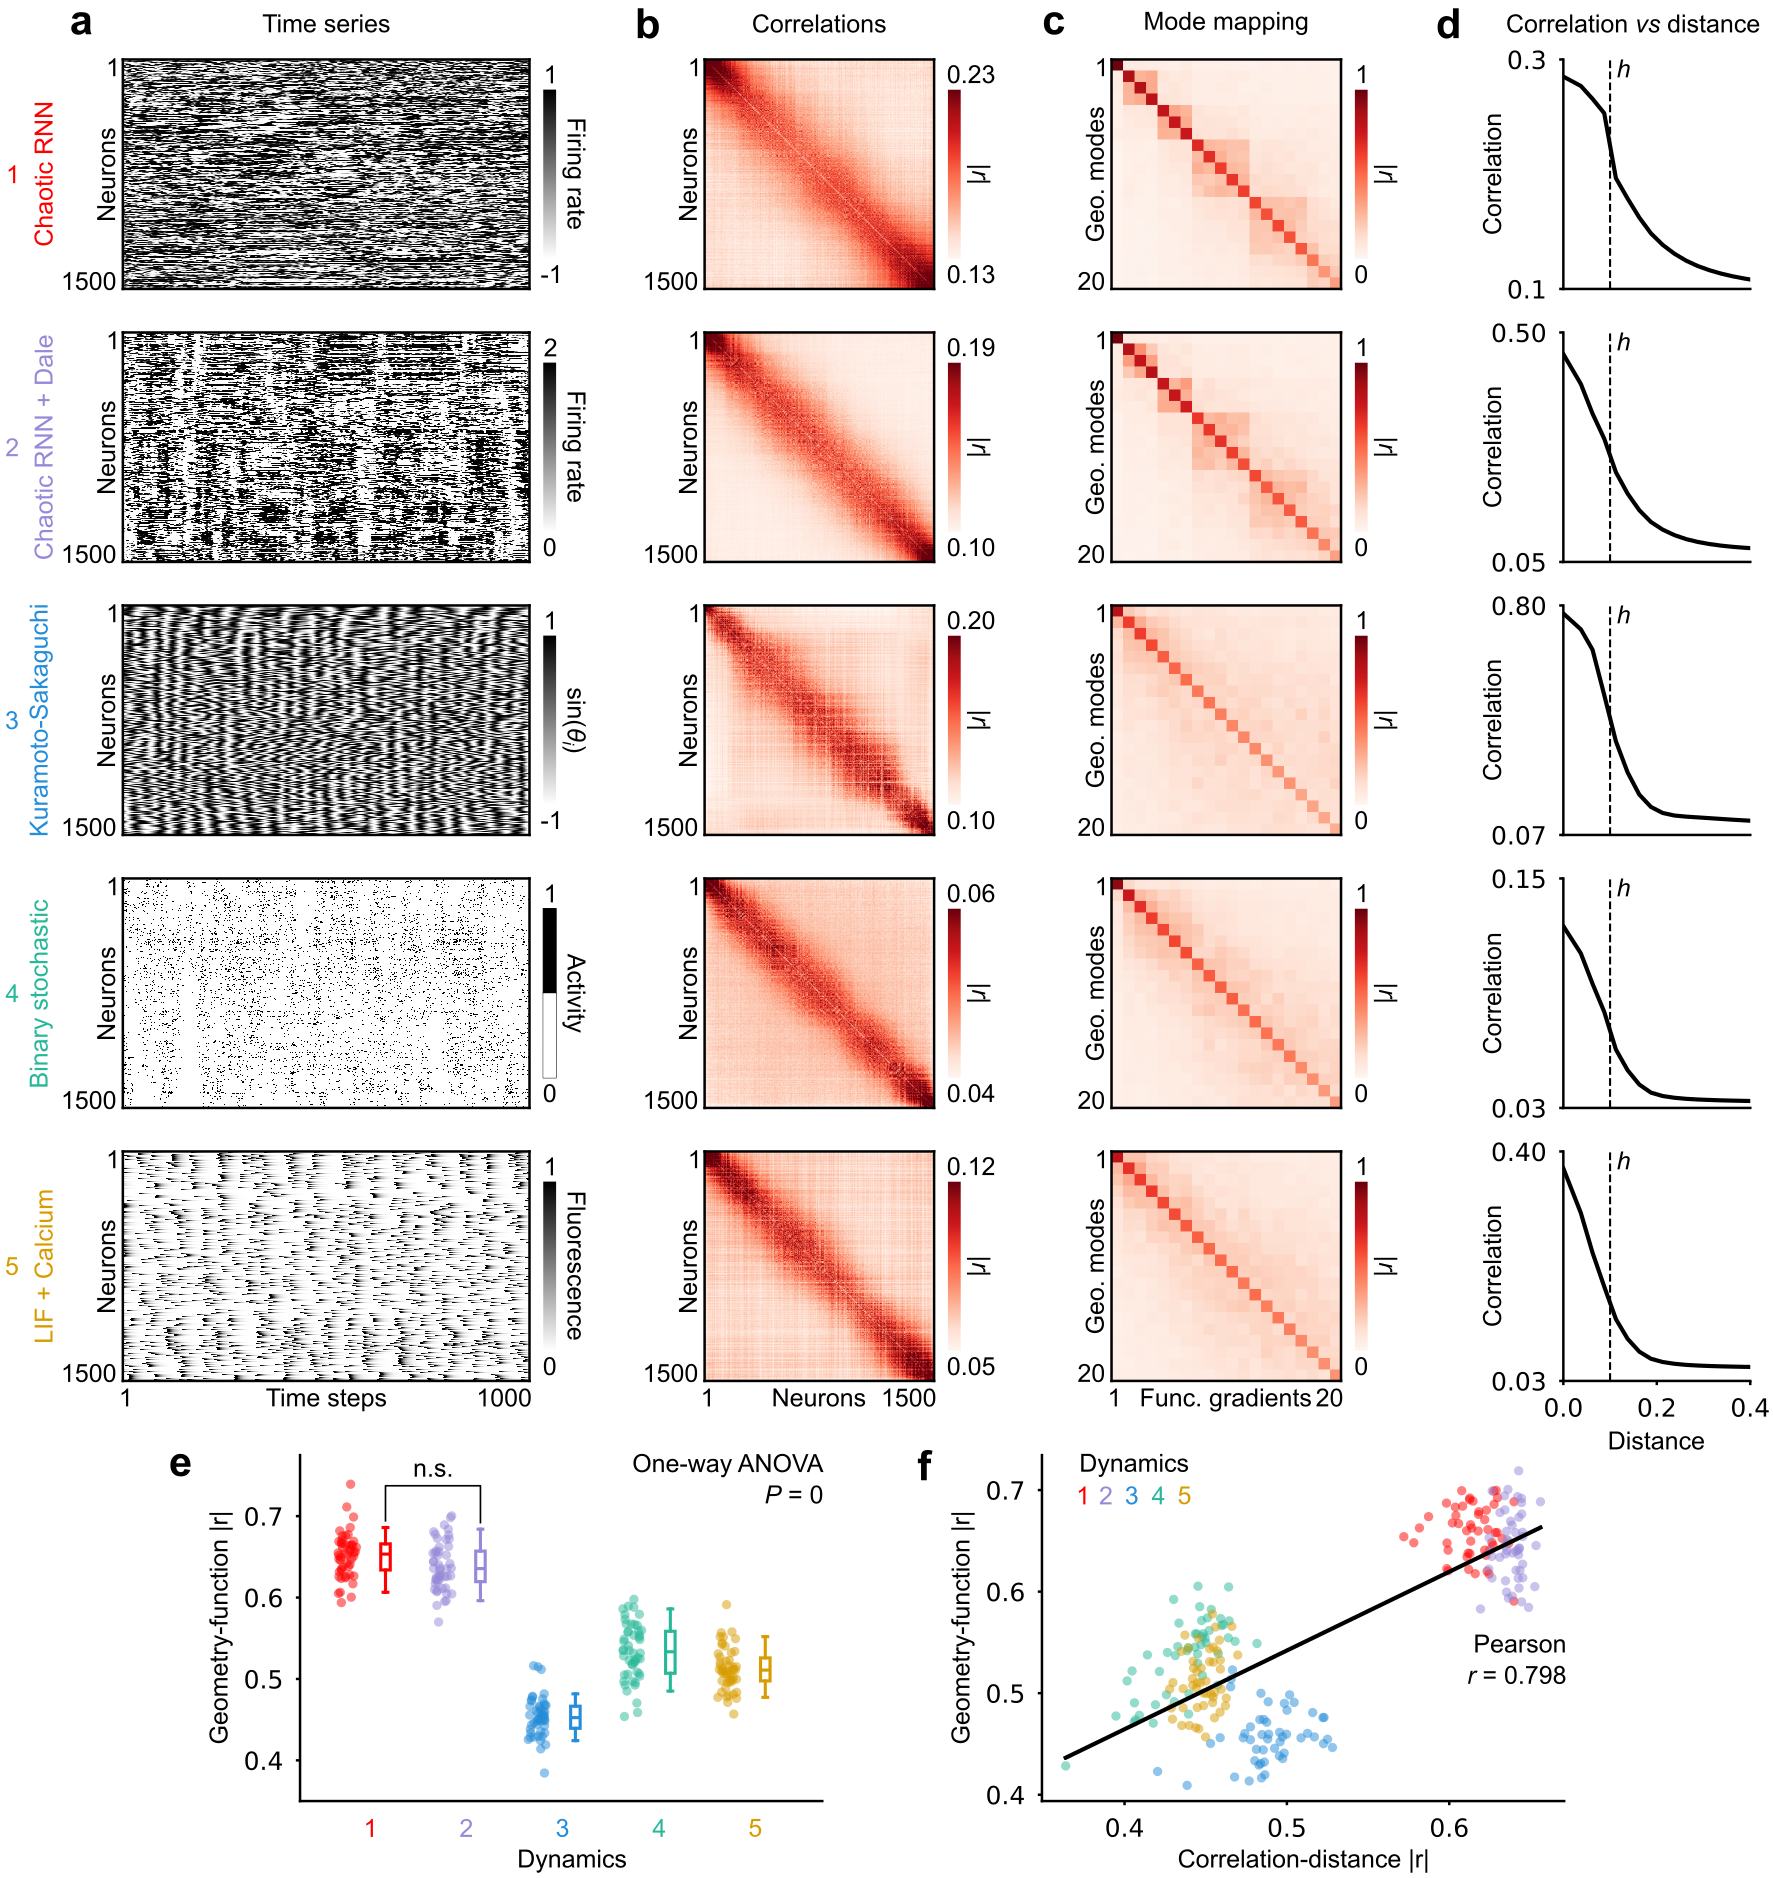
\includegraphics[width=1.0\linewidth]{figures/supp_dynamics.png}
    \caption{Geometry-function mapping in ellipsoid for different dynamical systems. (\textbf{a}) Example simulated time series from five dynamical models, indicated on the left and detailed in Methods; all simulations are embedded in the ellipsoid geometry. (\textbf{b}) Example pairwise neuronal activity correlations for each model, averaged across 100 simulations; the matrix is sorted to follow the $z$ axis of the ellipsoid. (\textbf{c}) Gradient-eigenmode similarity matrices for each dynamical model, averaged across 10 ellipsoids. (\textbf{d}) Average correlation-distance relationships for each dynamical model; a dashed line indicates the connectivity radius $h$ of neurons. (\textbf{e}) Average gradient-eigenmode correlations for each dynamical model (50 different simulations, averaged over mode pairs); different models yield statistically different geometric mappings (one-way ANOVA, $P=0$). (\textbf{f}) Geometry-function $|r|$ as a function of the correlation-distance $|r|$ for the five different models; dynamical models whose correlations are more tightly coupled to euclidean distance yield better geometric gradients (Pearson $r=0.798$), which suggests that dynamics with many spurious or long-range correlations degrade the geometric mapping. }
    \label{supp_dynamics}
\end{figure*}

\newpage

\begin{figure*}[t]
    \centering
    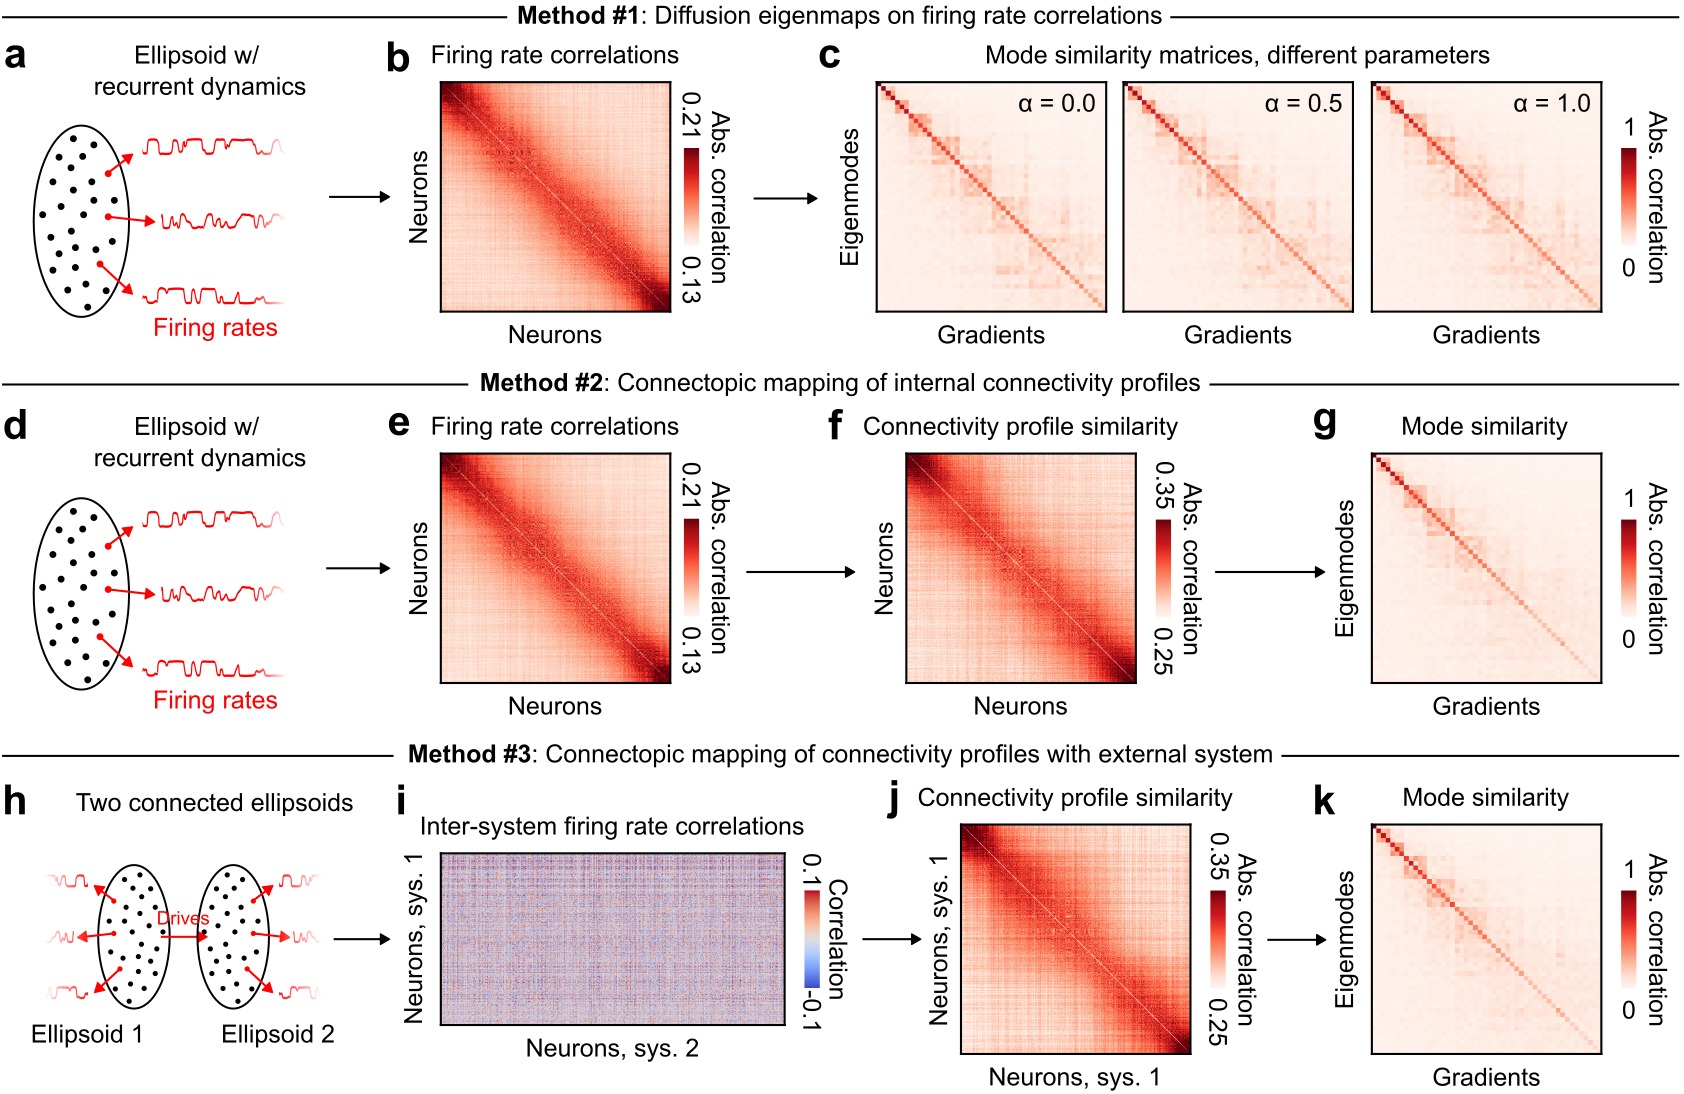
\includegraphics[width=1.0\linewidth]{figures/supp_gradient_methods.png}
    \caption{Derivation of geometric gradients using various gradient analysis methods. (\textbf{a}-\textbf{c}) Method 1 uses the diffusion maps algorithm on the firing rate correlation matrix to compute gradients, yielding results that are mostly independent of the $\alpha$ parameter controlling the effect of local density on the diffusion process. (\textbf{d}-\textbf{g}) Method 2 adds one extra step to the first method by computing the connectivity profile similarity from the correlation matrix before computing gradients. (\textbf{h}-\textbf{i}) Method 3 approximates the connectopic mapping procedure used in Pang et al, who derived subcortical gradients from their temporal association with cortical activity. Here, two interconnected systems are simulated, one smaller representing a subcortical region, and one larger representing external regions like the cortex. Time series from both ellipsoids are correlated to each other, and then the connectivity profile similarity matrix is used to compute gradients. Overall, this supplementary analysis demonstrates that geometric gradients can be obtained from gradient derivation methods that vary in their sequence of numerical operations, highlighting their methodological robustness.}
    \label{supp_methods}
\end{figure*}

\newpage

\begin{figure*}[t]
    \centering
    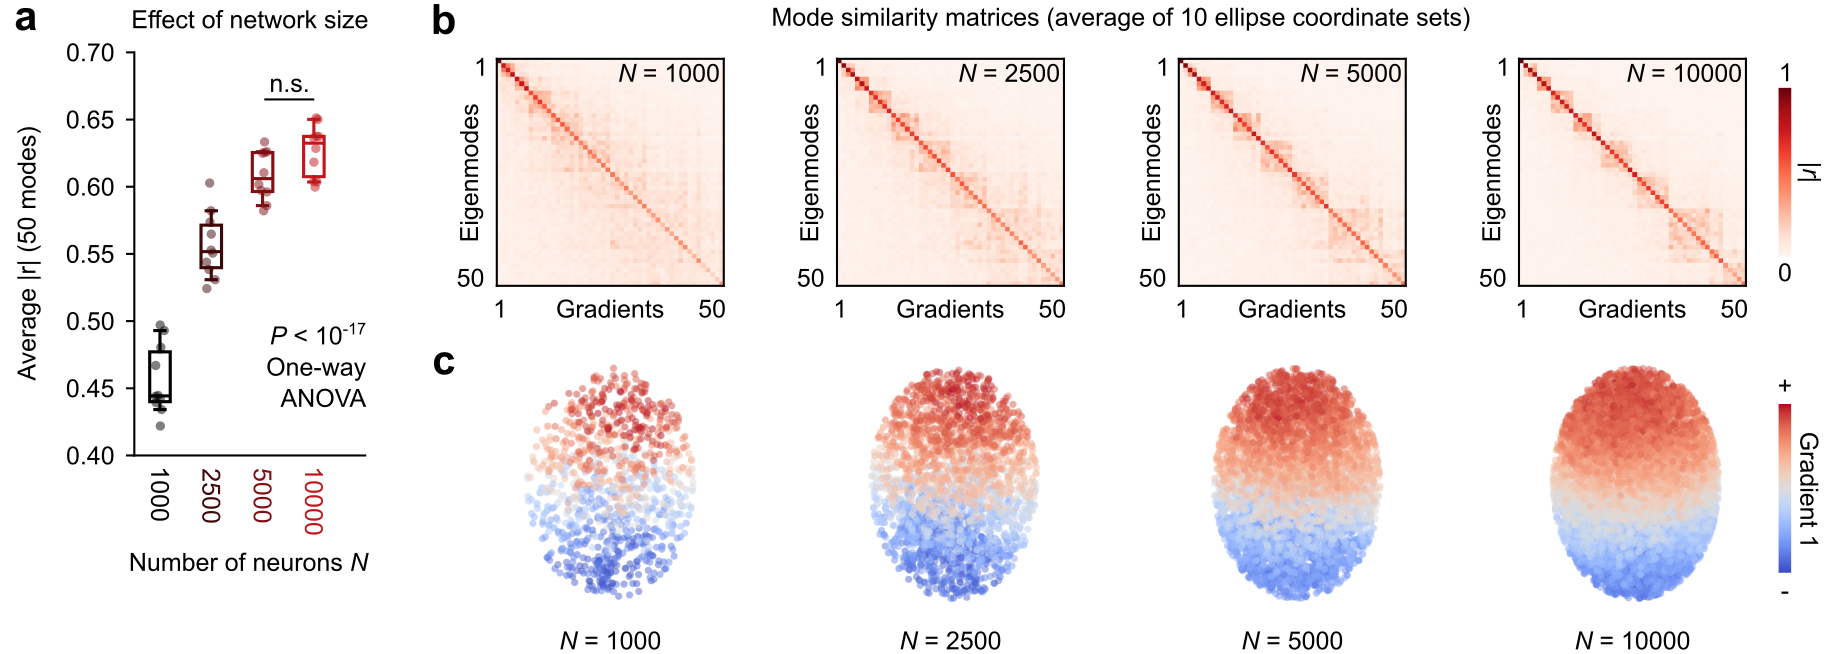
\includegraphics[width=1.0\linewidth]{figures/supp_network_size.png}
    \caption{Geometry-function mapping in ellipsoid for different network sizes. (\textbf{a}) Average gradient-mode similarity (averaged over 50 mode pairs) for four different network sizes; denser networks exhibit gradients that correlate more with geometric eigenmodes (one-way ANOVA, $P<10^{-17}$). (\textbf{b}) Gradient-eigenmode similarity matrices for different network sizes (indicated in the top right matrix corners), averaged over 10 ellipsoids. (\textbf{c}) Neuron centroids colored by the numerical values of the first functional gradient for increasing network sizes.}
    \label{supp_network_size}
\end{figure*}

\newpage

\begin{figure*}[t]
    \centering
    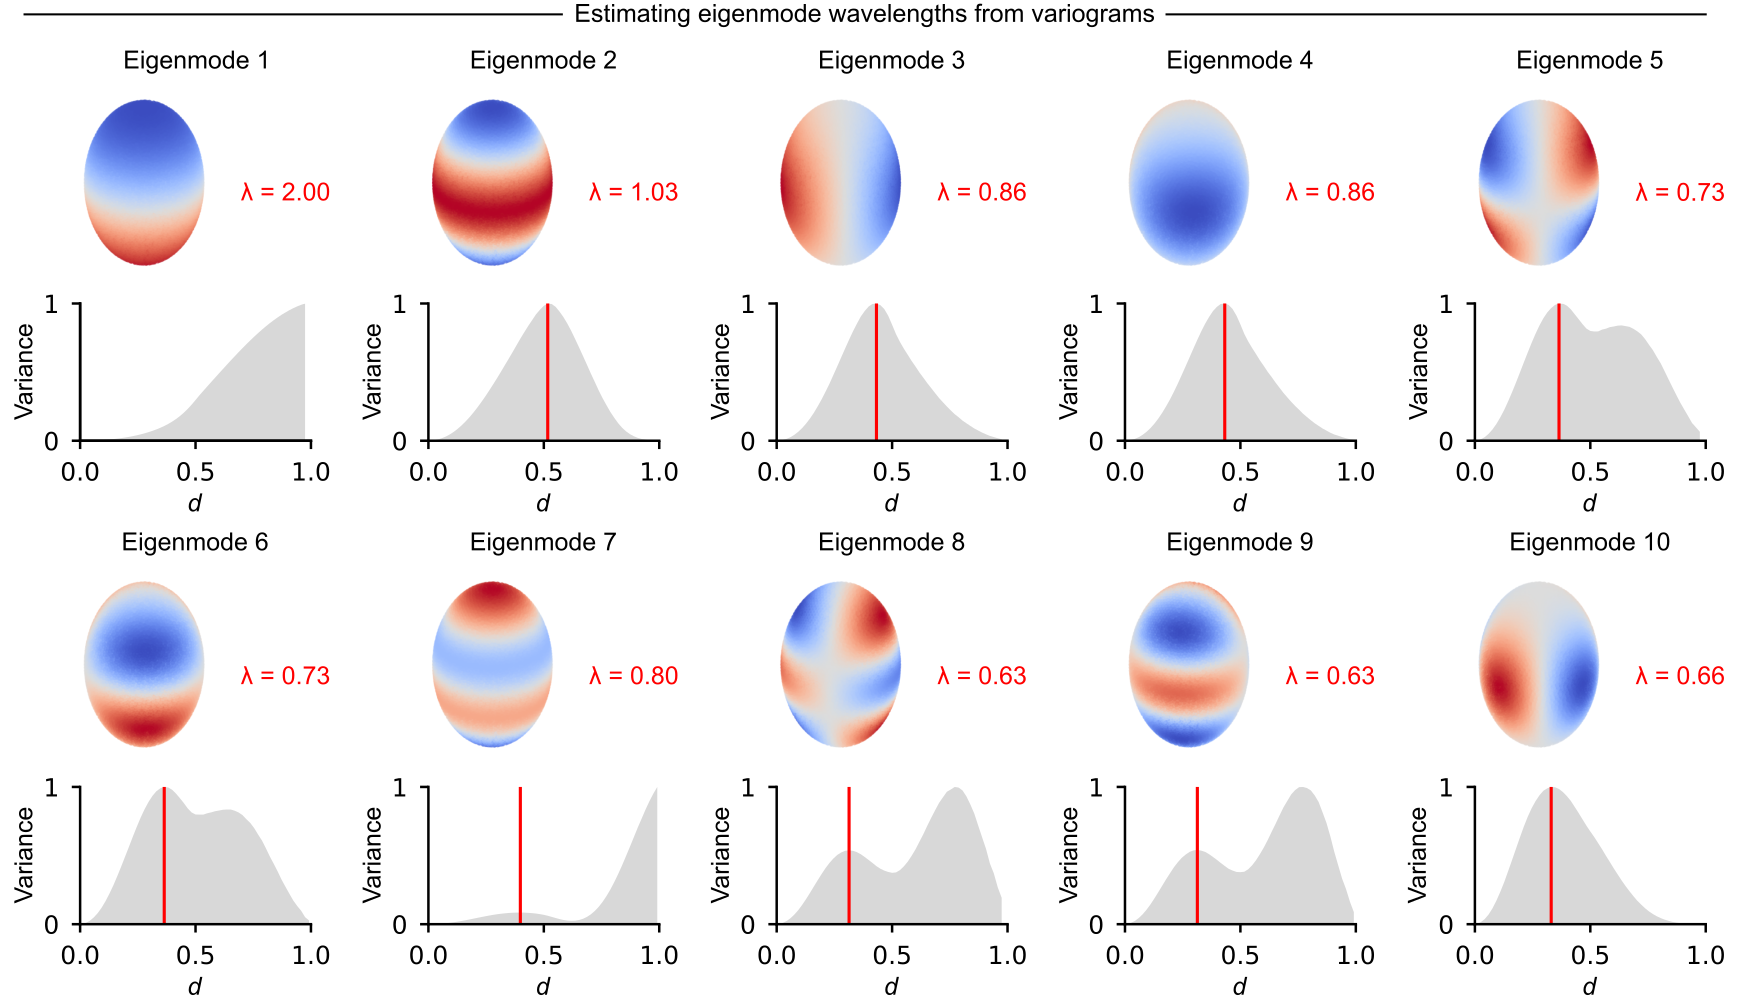
\includegraphics[width=1.0\linewidth]{figures/supp_variograms.png}
    \caption{Estimating eigenmode wavelengths using their spatial variograms. The first 10 ellipsoid eigenmodes are plotted alongside their wavelengths (top rows), which are estimated from the first peak of each variogram (bottom rows, Methods).}
    \label{supp_variograms}
\end{figure*}

\newpage

\begin{figure*}[t]
    \centering
    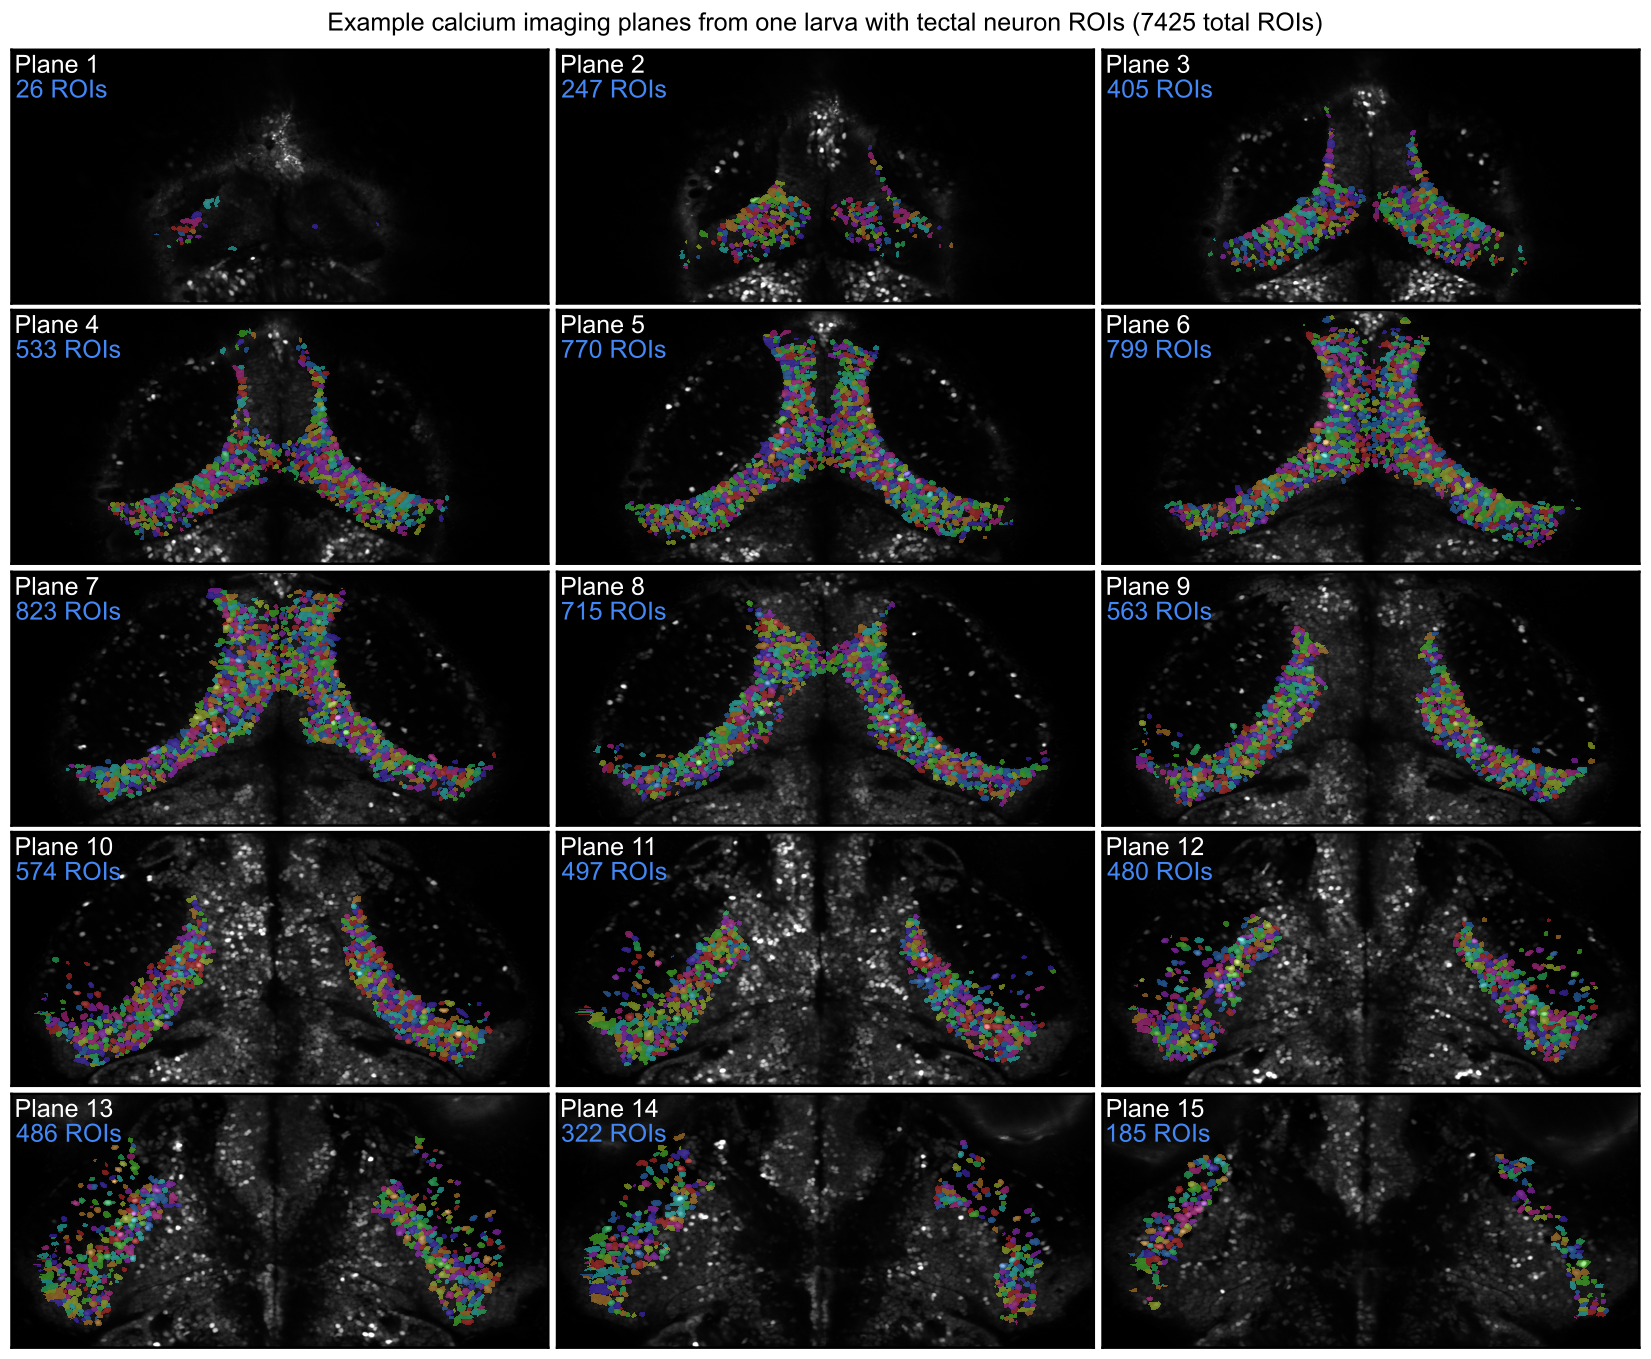
\includegraphics[width=1.0\linewidth]{figures/supp_imagingplanes.png}
    \caption{Temporal averages of two-photon calcium imaging planes from one example animal, with pseudocolored nuclei located within the optic tectum identified using Cellpose 2.0. The number of detected regions of interest (ROIs) is indicated on each plane. Imaging volumes extend from the most dorsal (top left) to the most ventral (bottom right) parts of the tectum across both hemispheres to ensure that the entire 3D structure is properly sampled.}
    \label{supp_imagingplanes}
\end{figure*}

\newpage

\begin{figure*}[t]
    \centering
    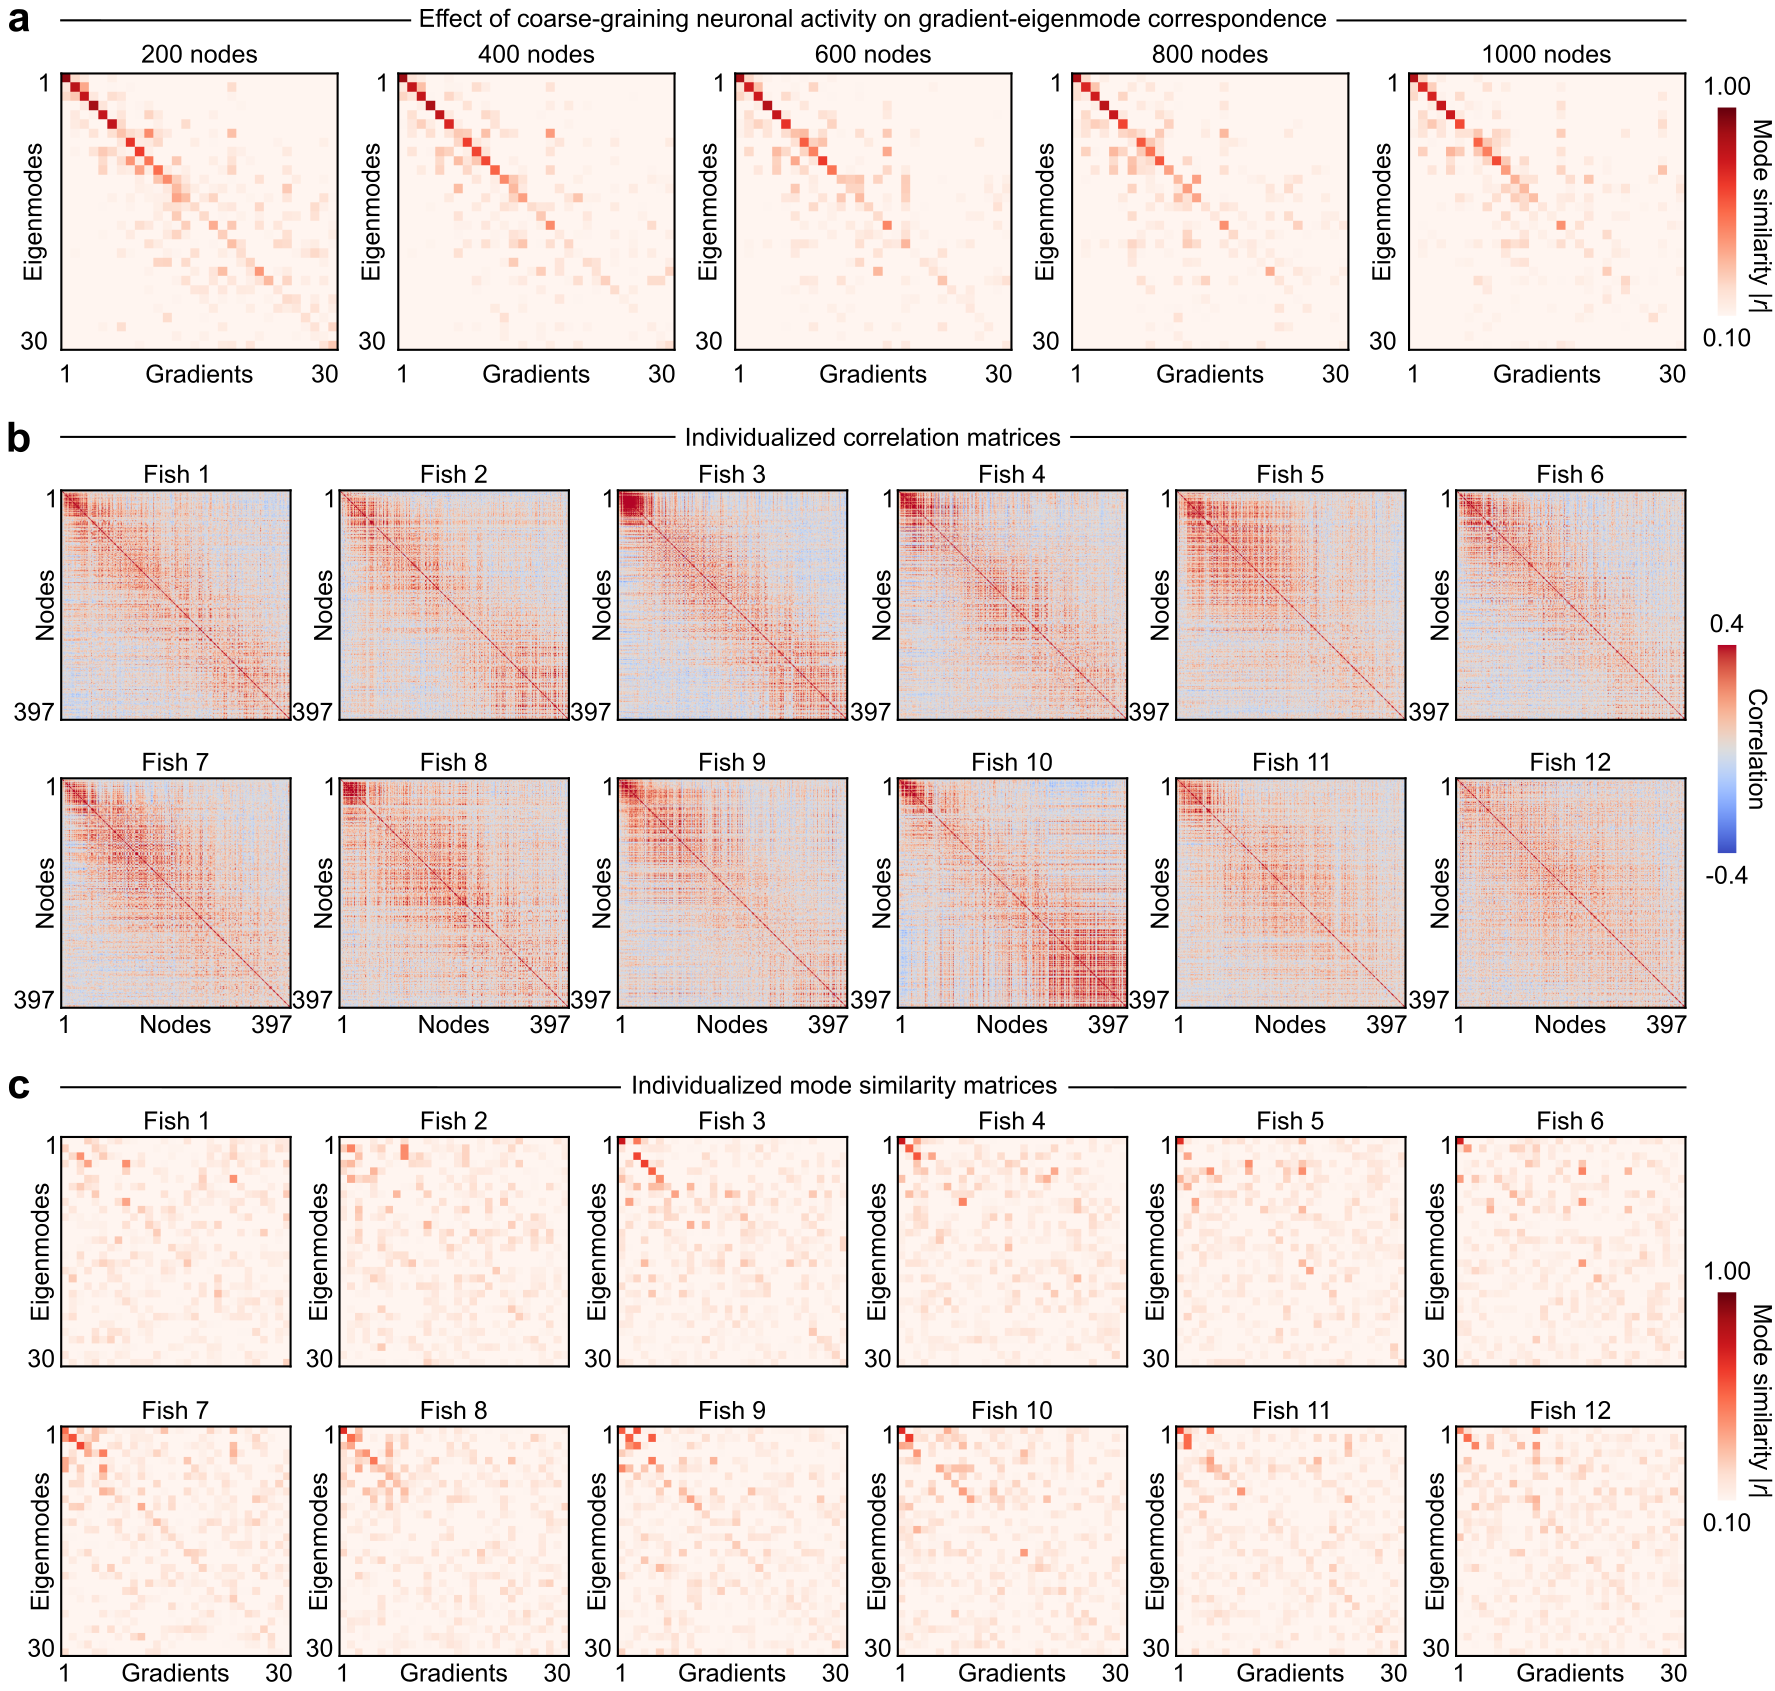
\includegraphics[width=1.0\linewidth]{figures/supp_coarsegraining.png}
    \caption{Effect of coarse-graining and averaging on geometric gradients. (\textbf{a}) Gradient-eigenmode similarity matrices for varying numbers of network nodes in the optic tectum; notice the minimal effect of spatial resolution on the mapping quality. (\textbf{b}) Correlation matrices of optic tectum node activity for 12 different larvae, sorted from anterior to posterior nodes. (\textbf{c}) Gradient-eigenmode similarity matrices calculated on the individual correlation matrices from the previous panel; notice the poor quality of the mapping in most animals. This suggests that individual imaging sessions insufficiently sample the correlation structure of the optic tectum.}
    \label{supp_coarsegraining}
\end{figure*}

\newpage

\begin{figure*}[t]
    \centering
    \includegraphics[width=1.0\linewidth]{figures/supp_noise.png}
    \caption{Influence of experimental noise on the geometric cutoff wavelength. (\textbf{a}) Five example single-neuron fluorescence time series, with varying noise levels; black, raw traces; red, raw traces with numerical noise drawn from a normal distribution with 3 times the standard deviation of the data. (\textbf{b}) Absolute correlation $|r|$ averaged across 30 eigenmode-gradient pairs for varying noise levels applied to fluorescence time series; red, average curve; black dots, 10 replicates per noise level. (\textbf{c}) Cutoff wavelength inferred from a piecewise linear fit on mode correlation matrix diagonals for varying noise levels; red, average curve; black dots, 10 replicates per noise level; despite a gradual decrease of correlations observed in $\textbf{b}$, no significant cutoff wavelength differences are observed until noise levels reach $3.5\sigma_{\text{data}}$ (One-way ANOVA, $P=0.105$, $F=1.929$). This analysis suggests that experimental noise has a negligible influence on the position of the cutoff point in the eigenmode-gradient mapping.}
    \label{supp_noise}
\end{figure*}

\newpage

\begin{figure*}[t]
    \centering
    \includegraphics[width=1.0\linewidth]{figures/supp_tectum_cutoff.png}
    \caption{Two different methods can retrieve the connectivity radius $h$ of the optic tectum based on numerical simulations. (\textbf{a}) Method 1 identifies cutoff points at the level of individual eigenmodes by varying the connectivity radius $h$ over many simulations, which generates curves with abrupt drop-offs for each eigenmode; this approach is used in Fig. \ref{fig3}. (\textbf{b}) The $h$ cutoff points identified for each eigenmode using method 1 are linearly correlated to eigenmode spatial wavelengths (averaged over 10 coordinate sets, 100 simulations per set). (\textbf{c}) In contrast, method 2 identifies cutoff points at the mode ensemble level, rather than per individual eigenmode. This is achieved by fitting a piecewise linear relationship to the gradient-eigenmode similarity matrix diagonal, with the elbow of the curve corresponding to the cutoff point. (\textbf{d}) Cutoff points identified using this method are also linearly correlated with the connectivity radius $h$ used in simulations (averaged over 10 coordinate sets, 100 simulations per set). While method 1 can only be applied to numerical simulations, method 2 is applicable to real data, as it requires a single mode similarity matrix to estimate the $h$ parameter, provided a linear relationship has been established from numerical simulations beforehand. This approach is used in Fig. \ref{fig7} to estimate the arbor size of tectal neurons.}
    \label{supp_tectum_cutoff}
\end{figure*}

\newpage

\begin{figure*}[t]
    \centering
    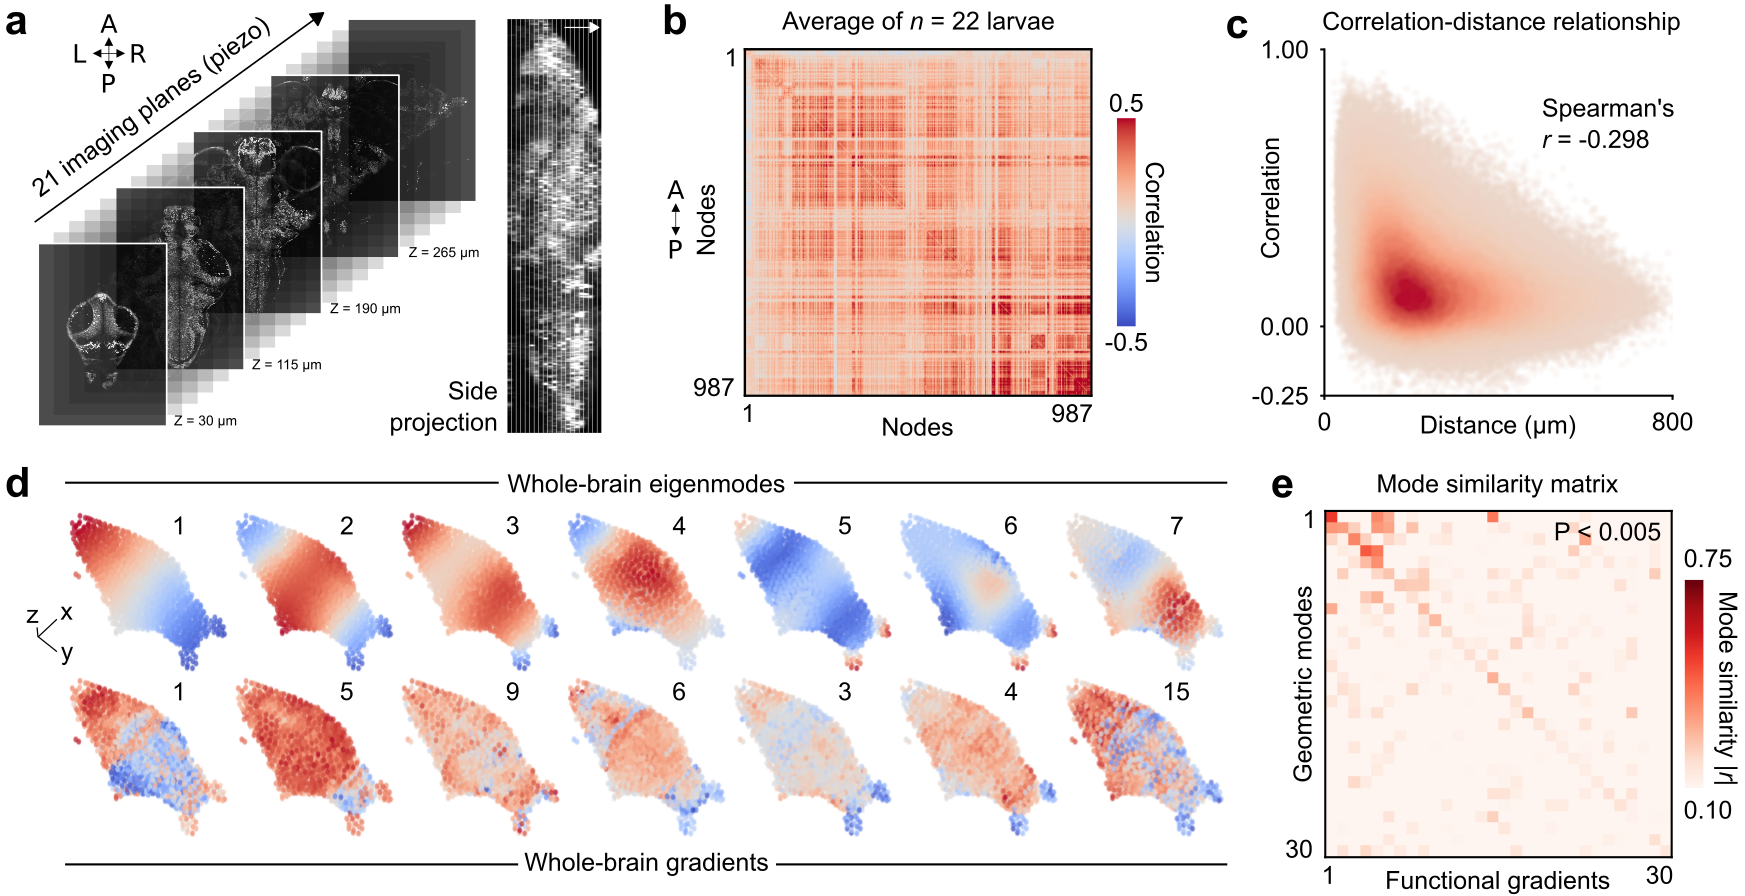
\includegraphics[width=1.0\linewidth]{figures/supp_wholebrain.png}
    \caption{Whole-brain functional connectivity gradients do not reflect geometric eigenmodes. (\textbf{a}) Whole-brain imaging using two-photon microscopy; the dataset and imaging parameters are described in a previous study. (\textbf{b}) Group-averaged whole-brain functional connectivity ($n=22$ larvae, 5-7 days post-fertilization, 10 minutes of spontaneous activity); neurons are mapped in 987 nodes per hemisphere, and correlations are averaged across hemispheres. (\textbf{c}) Correlation-distance relationship of whole-brain FC (Spearman's $r=-0.298$). (\textbf{d}) Top, whole-brain geometric eigenmodes; bottom, whole-brain functional connectivity gradients; both mode ensembles are projected onto 987 nodes per brain hemisphere and colors are scaled arbitrarily. (\textbf{e}) Whole-brain gradient-eigenmode similarity matrix; the mapping quality is significant at the group level, that is, when mode correlations are averaged over the matrix diagonal ($P<0.005$, 1000 SA-preserving spatial permutations). Nevertheless, the gradient-eigenmode mapping is substantially worse at the whole-brain level than within the optic tectum.}
    \label{supp_wholebrain}
\end{figure*}

\newpage

\begin{figure*}[t]
    \centering
    \includegraphics[width=1.0\linewidth]{figures/supp_smoothing.png}
    \caption{Spatial filtering drives geometric eigenmodes in both optic tectum and whole-brain calcium imaging data. (\textbf{a}) Tectal (top) and whole-brain (bottom) activity correlation matrices for varying spatial filtering kernel sizes, indicated on each matrix ($n=12$ larvae for tectal data, $n=22$ larvae for whole-brain data). (\textbf{b}) Gradient-eigenmode similarity $|r|$ averaged over 30 mode pairs for the optic tectum (red) and the entire brain (black). While numerical simulations in Fig. \ref{fig5} demonstrate potentially nonlinear effects of spatial filtering, this procedure immediately increases the gradient correspondence with geometric eigenmodes in real data.}
    \label{supp_smoothing}
\end{figure*}

\end{document}